% CAST MANUAL LATEX
% This is the official manual for the CAST program package
\documentclass[10pt,a4paper]{article} %DOCUMENTCLASS

%%%% PACKAGES
\usepackage[utf8]{inputenc} %ENCODING
\usepackage[english]{babel} %ENGLISH LANGUAGE STYLE
\usepackage[parfill]{parskip} %PARAGRAPH SPACING
\usepackage{color} %COLOURS
\usepackage{amsmath} %math
\usepackage{bm} %VECTOR BOLD AND ITALIC
\usepackage{longtable} %table over more than one page
\usepackage{listings} %ENABLE (SOURCE) CODE LISTINGS
%\usepackage{underscore} %AUTOMATICLY ESCAPING UNDERSCORES
\usepackage{graphicx} %LATEX CANT MANAGE IMAGES, SO WE NEED THIS
\usepackage{hyperref} %ENABLE URL SUPPORT
\usepackage{todonotes} % add TODO notes, use option [disable] to not show them
\usepackage[backend=biber,style=chem-angew,biblabel=dot]{biblatex} %REFERENCES
\addbibresource{castmanualReferences.bib} %ADD BIBLATEX REFERENCES FILE.
\usepackage{acronym} %SUPPORT FOR ABBREVIATIONS

\makeatletter % code for fixing bug in biblatex, see: http://tex.stackexchange.com/questions/311426/bibliography-error-use-of-blxbblverbaddi-doesnt-match-its-definition-ve 
\def\blx@maxline{77}
\makeatother


%%%%OPTIONS FOR CODE LISTINGS
\lstset{ %
	backgroundcolor=\color{white},   % choose the background color; you must add \usepackage{color} or \usepackage{xcolor}
	basicstyle=\footnotesize,        % the size of the fonts that are used for the code
	breakatwhitespace=false,         % sets if automatic breaks should only happen at whitespace
	breaklines=true,                 % sets automatic line breaking
	%captionpos=b,                    % sets the caption-position to bottom
	frame=single,	                 % adds a frame around the code
	keepspaces=true,                 % keeps spaces in text, useful for keeping indentation of code (possibly needs columns=flexible)
	%language=Octave,                 % the language of the code
	numbers=left,                    % where to put the line-numbers; possible values are (none, left, right)
	numbersep=5pt,                   % how far the line-numbers are from the code 
	showspaces=false,                % show spaces everywhere adding particular underscores; it overrides 'showstringspaces'
	showstringspaces=false,          % underline spaces within strings only
	showtabs=false,                  % show tabs within strings adding particular underscores
	stepnumber=1,                    % the step between two line-numbers. If it's 1, each line will be numbered
	tabsize=2,	                     % sets default tabsize to 2 spaces	
}

%%%%AUTHOR INFORMATION
\title{CAST Manual}
\author{Working Group Engels \\
	Julius-Maximilians Univeristy Wuerzburg \\
	Wuerzburg, Germany}
	

\begin{document}
\pagenumbering{Roman}
	%%%%%%%%%%%%%%%%%%%%%%%%%%%%%%%%%%%%
	%%%%                            %%%%
	%%%%     TITLE PAGE             %%%%
	%%%%                            %%%%
	%%%%%%%%%%%%%%%%%%%%%%%%%%%%%%%%%%%%

	% FRONT PAGE
\begin{center} 
	{\LARGE {\Huge \textbf{CAST}} \\ \vspace{1cm} Conformational Search and Analysis Tool}

    \todo[inline]{STILL STUFF MISSING! (todonotes, see next page)}
    
    \vspace{1cm}
	Version 3.1 \\
	\today
    \vspace{2cm}
	
\includegraphics[width=\textwidth]{img/CAST_CMYK_small.png}
	\end{center}

	%%%%%%%%%%%%%%%%%%%%%%%%%%%%%%%%%%%%
    %%%%                            %%%%
    %%%%        LIST OF TODOS       %%%%
    %%%%                            %%%%
    %%%%%%%%%%%%%%%%%%%%%%%%%%%%%%%%%%%%

    \newpage
    \listoftodos[TODOs for Manual]

	%%%%%%%%%%%%%%%%%%%%%%%%%%%%%%%%%%%%
	%%%%                            %%%%
	%%%%     TABLE OF CONTENTS      %%%%
	%%%%                            %%%%
	%%%%%%%%%%%%%%%%%%%%%%%%%%%%%%%%%%%%
	\newpage
	\tableofcontents

	%%%%%%%%%%%%%%%%%%%%%%%%%%%%%%%%%%%%
	%%%%                            %%%%
	%%%%     LIST OF FIGURES        %%%%
	%%%%                            %%%%
	%%%%%%%%%%%%%%%%%%%%%%%%%%%%%%%%%%%%

	\newpage
	\listoffigures

	%%%%%%%%%%%%%%%%%%%%%%%%%%%%%%%%%%%%
	%%%%                            %%%%
	%%%%     LIST OF TABLES         %%%%
	%%%%                            %%%%
	%%%%%%%%%%%%%%%%%%%%%%%%%%%%%%%%%%%%
	%\newpage
	% We don't need this right now
	%\listoftables
	
	%%%%%%%%%%%%%%%%%%%%%%%%%%%%%%%%%%%%
	%%%%                            %%%%
	%%%%     LIST OF ABBREVIATIONS  %%%%
	%%%%                            %%%%
	%%%%%%%%%%%%%%%%%%%%%%%%%%%%%%%%%%%%
	\section{Table of Abbreviations}
	\begin{acronym}[DEINEMUDDA] % längste Abkürzung steht in eckigen Klammern
		\setlength{\itemsep}{-\parsep} % geringerer Zeilenabstand
		\acro{AMBER}{Assisted Model Building with Energy Refinement}
		\acro{AMOEBA}{Atomic Multipole Optimized Energetics for Biomolecular Applications}
		\acro{CAST}{Conformational Analysis and Search Tool}
		\acro{CHARMM}{Chemistry at Harvard Macromolecular Mechanics}
		\acro{DFT}{Density Functional Theory}
		\acro{DFTB}{Density Functional Tight Binding}
		\acro{DOF}{degree of freedom}
		\acrodefplural{DOF}[DOFs]{degrees of freedom}
		\acro{dRMSD}{distance root-mean-square deviation}
		\acro{DS}{Diversification Search}
		\acro{FEP}{Free Energy Pertubation}
		\acro{GAFF}{General Amber Force Field}
		\acro{GCC}{GNU Compiler Collection}
		\acro{GPU}{graphics processing unit}
		\acro{LAPACK}{Linear Algebra PACKage}
		\acro{MC}{Monte-Carlo}
		\acro{MCM}{Monte-Carlo with Minimization}
		\acro{MD}{Molecular Dynamics}
		\acro{MOPAC}{Molecular Orbital Package}
		\acro{MPI}{Message Parsing Interface}
		\acro{NEB}{Nudged Elastic Band}
		\acro{NMR}{nuclear magnetic resonance}
		\acro{OPLS-AA}{Optimized Potentials for Liquid Simulations All-Atoms}
		\acro{PBC}{Periodic Boundary Conditions}
		\acro{PCA}{Principal Component Analysis}
		\acro{PDF}{probability density function}
		\acro{PES}{potential energy surface}
		\acro{RMSD}{root-mean-square deviation}
		\acro{SAPT-FF}{Symmetry Adapted Perturbation Theory based Force Field}
		\acro{TS}{Tabu Search}
		\acro{US}{Umbrella Sampling}
		\acro{VdW}{Van-der-Waals}
		\acro{VMD}{Visual Molecular Dynamics}
		\acro{WHAM}{Weighted Histogram Analysis Method}
	\end{acronym}
	\newpage
	
		%%%%%%%%%%%%%%%%%%%%%%%%%%%%%%%%%%%%
	%%%%                            %%%%
	%%%%     PREFACE                %%%%
	%%%%                            %%%%
	%%%%%%%%%%%%%%%%%%%%%%%%%%%%%%%%%%%%
	\pagenumbering{arabic}
	\section{Preface}
	The \ac{CAST} allows the accurate treatment of large and flexible (macro-)molecular systems. For the determination of thermally accessible minima \ac{CAST} offers the newly developed \ac{TS} algorithm \supercite{tabusearch}, as well as \ac{MC}\supercite{mc_original}, \ac{MCM}\supercite{MCM_original} and \acf{MD}\supercite{computer_simulation_of_MD} implementations. For the determination of reaction paths \ac{CAST} provides the PathOpt\supercite{pathopt}, the \ac{NEB}\supercite{neb_original} and the \ac{US}\supercite{umbrella_sampling} approach. Access to free energies is possible through the \ac{FEP} approach. Along with a number of standard force fields, a newly developed Symmetry Adapted Perturbation Theory based force field (\acs{SAPT-FF}) is included. There are also interfaces to different external programs for Semi-Empirical computations (e.\,g. DFTB\textsuperscript{+}\supercite{dftb} or MOPAC\supercite{mopac, mopac_parallel}) and for quantum chemistry methods (e.\,g. TeraChem\supercite{terachem} or Gaussian). For more information on \ac{CAST} see \cite{cast}.
	\newpage
	
	
	%%%%%%%%%%%%%%%%%%%%%%%%%%%%%%%%%%%%
	%%%%                            %%%%
	%%%%     COMPILING CAST         %%%%
	%%%%                            %%%%
	%%%%%%%%%%%%%%%%%%%%%%%%%%%%%%%%%%%%
	\section{Compiling CAST} \label{sec:compile}
	The \ac{CAST} source code is published at \url{https://github.com/AKEngels/CAST}. There is a \textit{premake5} configuration file included to automatically generate makefiles as well as Visual Studio solutions. See \url{https://premake.github.io/} for more information on premake.
	
	Compiling \ac{CAST} with the standarf openMP flags enables multithreading.
	
	For matrix-operations \ac{CAST} is able to use \ac{LAPACK} via armadillo (\url{http://arma.sourceforge.net/}). The premake5-lua-script includes predefined configurations that enable LAPACK. 
	
	Some parts of \ac{CAST} also use python modules or interfaces to perform calculations. The version of python you need to install before the compilation of CAST is 2.7. You also have to install the python modules that are needed for the task you desire. Compiling CAST with python enabled can also be done by premake. Choose the configuration Python\_Release or Python\_Debug. If you have a 32bit version of python installed you can only compile \ac{CAST} in 32bit mode, if you have python 64bit you can only compile \ac{CAST} in 64bit mode. 
	
	\textbf{For users on ECPC or UNICORN:} CAST is installed in the folder /apps/CAST/. Submit scripts to submit a job with CAST (``normal'', with python or with armadillo) are also provided in that folder. If it is important for you to use the newest CAST version run the script update.sh in the folder /apps/CAST/CAST as a sudo user or ask someone with the sudo password to do it for you.

	
	\newpage
	%%%%%%%%%%%%%%%%%%%%%%%%%%%%%%%%%%%%
	%%%%                            %%%%
	%%%%       Installation         %%%%
	%%%%                            %%%%
	%%%%%%%%%%%%%%%%%%%%%%%%%%%%%%%%%%%%

	\section{Installation}
	At the moment there are no precompiled executables of \ac{CAST} provided online so you have to clone the github repository (\url{https://github.com/AKEngels/CAST}) and compile the code by yourself. You can get hints about how to do that from the wiki entry ``How to build CAST''. Be aware that the default branch of the repository is the devel branch but the latest stable release is the master branch.

	\newpage
	
	\section{First Steps}
	
	If you use \ac{CAST} for the first time consider looking at the CAST tutorial which can also be found on the github repository:\\ \url{https://github.com/AKEngels/CAST/tree/master/manual/Tutorial/LaTeX}
	
	\newpage

	%%%%%%%%%%%%%%%%%%%%%%%%%%%%%%%%%%%%%%
	%%%%                              %%%%
	%%%% General Structure and Useage %%%%
	%%%%                              %%%%
	%%%%%%%%%%%%%%%%%%%%%%%%%%%%%%%%%%%%%%
	\section{General Structure and Usage}
	\ac{CAST} features several main computation methods which can be combined with force fields, semi-empirical or \ac{DFT} methods via several interfaces. Input file formatting and available commands are discussed in the following paragraphs.


	%%%% Configuration File %%%%
	\subsection{Configuration File}
	A file named either \glqq CAST.txt\grqq~or \glqq INPUTFILE\grqq~can be used to specify the configuration options of \ac{CAST}\footnote{If both files are present, \glqq CAST.txt\grqq~will be read.}. By starting the CAST executable with the commandline-switches \glqq -s\grqq~or \glqq -setup\grqq~an alternative configuration file can be specified\footnote{Call either as \glqq CAST.exe -s filename.txt\grqq~or as \glqq CAST.exe -setup=filename.txt\grqq~. The configuration file has to be placed in the same folder as the CAST executable.}. It contains option keywords followed by one or more appropriate values. The keywords are case sensitive. Comments can be included by starting the line with a \glqq \#\grqq. The variables are usually of type integer, floating point or boolean (booleans currently being either \glqq 0\grqq~and \glqq 1\grqq~or plain text \glqq true\grqq~and \glqq false\grqq~without quotation marks).\\

	The following input commands are compulsory for \ac{CAST} to work and have to be set for every calculation.\\~\\
	\begin{minipage}{\textwidth}
	\begin{longtable}{|p{3cm}|p{5cm}|p{3cm}|}
		Variable&	Effect &	Default \\
		\hline
		verbosity &	Amount of \ac{CAST} output &	1\\
		cores &	Number of OpenMP threads &	1\\
		name &	Name of input file &	none\\
		outname &	Name of output files &	none\\
		input-type &	Format of coordinate file &	TINKER\\
	\end{longtable}
	\end{minipage}
	
	The keyword for the path of the used coordinate file is "name". The variable ``cores'' controls the number of threads if multi-threated \ac{CAST} is used (i.e. if \ac{CAST} has been compiled with OpenMP\supercite{openmp08}). ``outname'' defines the name of the outputfile with information regarding the calculation.
	The switch controlling how much information \ac{CAST} will print to the console is named "verbosity". Proper values are positive integral numbers where low numbers indicate less information than higher numbers do. Suggested values for productive use are 1, 2 or 3. In general, lower numbers will yield less obvious output which is  more suitable for processing (since there are less superficial descriptors printed). Higher values may slow down program execution but provide detailed insight into the program's execution. The detailed effect of the numerical verbosity setting depends on the chosen task.

	An example input for a single point energy calculation with \ac{OPLS-AA} Force Field\supercite{oplsaa, oplsaa2} is given below:
	
	\begin{lstlisting}
	verbosity              3
	name                   inputstructure.xyz
	inputtype              TINKER
	outname                thisIsTheOutputFile
	cores                  4
	task                   SP
	interface              OPLSAA
	paramfile              oplsaa.prm\end{lstlisting}

	A more explicit, commented version of the INPUTFILE containing all parameters is distributed with \ac{CAST}.
		
	%%%% Force Fields %%%%
	\subsection{Force fields}
	\ac{CAST} features four different force field implementations:\\
	\begin{itemize}
	 \item \acf{OPLS-AA}\supercite{oplsaa, oplsaa2} \item \acf{CHARMM}\supercite{charmm}
	 \item \acf{AMBER}\supercite{amber}
	 \item \acf{AMOEBA}\supercite{amoeba_current, amoeba_current2}
	\end{itemize}~\\
	With the exception of the \ac{AMOEBA} force field, the non-bonded parts of the force fields have been parallelized using the OpenMP programming model. Furthermore, the \ac{FEP} and SPME \todo{smooth particle mesh ewald? - does it still exist???} methods can only be used with \ac{OPLS-AA}, \ac{CHARMM} and \ac{AMBER}. The force fields have to be in a format similar to the one used by the TINKER\supercite{tinker} program. They may be obtained from the TINKER\supercite{tinker} website.
		%% AMOEBA and short range correction
		\subsubsection{AMOEBA and short range correction}
The AMOEBA FF belongs to the class of polarizable FFs. The energy description should not be described in detail. A detailed description can be found in \cite{Ponder2010}  The SAPT-FF is a specialized kind of the AMOEBA FF, whereas the short-range electrostatics are treated within a partitioning scheme.
For the description of the electrostatic energy it is a common approach
to use a finite expansion over atomic multipoles. The simple multipole
expansion underestimates the electrostatic energy and for a better
description a penetration energy can be included by using the Coulombic
energy between pro molecular charge densities. The classical electrostatic
energy (Coulomb) between two molecules A and B is described by the
following expression,
\begin{equation}
E_{es}=\int\int\rho_{A}(r_{A})\rho_{B}(r_{B})|r_{A}-r_{B}|^{-1}dr_{A}dr_{B}\label{eq:Coulombic}
\end{equation}
where $\rho_{A}(r_{A})$ and $\rho_{B}(r_{B})$ are the molecular
charge distributions, containing nuclear and electronic contributions.
In most cases in computational work the electron distribution is approximated
by a set of multipole moments.\supercite{Stone1996} But it is shown that
they underestimate the exact energies which can be calculated by exact
integration methods. This is related due to the fact that the penetration
of the electronic distribution of molecule A inside molecule B is
not included in these approaches. 

The penetration energy is affected by the Coulombic charge density
between pro molecular charge distributions (atomic charge distributions),
which means that it is the dominant part. Therefore, the charge distribution
can be split into a sum of atomic and deformation terms. The atomic
charge distributions are described by spherical ones. In consequence
the Coulombic energy is relatively easy to compute. It can be calculated
as functions depending on the distance and several parameters. Then
the contribution term of atom A can be written in the following way\\supercite{Spackman1986a},
\begin{equation}
\rho_{A}(r_{A})=\sum_{i\in A}[\rho_{A,i}^{atomic}(r_{A})+\Delta\rho_{A,i}^{elec}(r_{A})]=\rho_{A}^{pro}(r_{A})+\Delta\rho_{A,i}^{elec}(r_{A})
\end{equation}
which describes the partitioning of the molecular electronic distribution.
The pro molecular charge distribution of spherical atom A is $\rho_{A}^{pro}(r_{A})$
and $\Delta\rho_{A,i}^{elec}(r_{A})$ is the deformation term. Now
it is possible to rewrite $E_{es}$ and fill in $\rho_{A}\rho_{B}$
in eq. \ref{eq:Coulombic} For this $\rho_{A}\rho_{B}$ is shown.
\[
\rho_{A}\rho_{B}=\sum_{i\in A}\sum_{j\in B}[\rho_{A,i}^{atomic}\rho_{B,i}^{atomic}+\rho_{B,j}^{atomic}\Delta\rho_{A,i}^{elec}+\rho_{A,i}^{atomic}\Delta\rho_{B,j}^{elec}+\Delta\rho_{A,i}^{elec}\Delta\rho_{B,j}^{elec}]
\]
\begin{equation}
=\rho_{A}^{pro}\rho_{B}^{pro}+\rho_{A}^{pro}\Delta\rho_{B}^{elec}+\rho_{B}^{pro}\Delta\rho_{A}^{elec}+\Delta\rho_{A}^{elec}+\Delta\rho_{B}^{elec}
\end{equation}
\\
In consequence $E_{es}$ can be expressed in three terms containing
pro molecule and deformation depending energies.
\begin{equation}
E_{es}=E_{pro-pro}+E_{pro-def}+E_{def-def}\label{Ees}
\end{equation}
The description with pseudo atomic spheres leads to zero multipole
moments for the spherical atom. Only the deformation term $E_{def-def}$
includes multipole moments. If no atomic multipole moments are used
all other terms are zero for spherical pseudoatoms, so it is necessary
to use an atomic description. This is the case for the Bader's atoms
in molecules (AIM) theory. There the electronic distribution is divided
into discrete atomic fragments. In the case of fitted charge/multipole
expansions derived from electrostatic potentials it would generally
work, but there are cases for which this approach fails. It is important
to know that there are many differences between the partitioning schemes
and how they are implemented. Especially the multipole expansion and
the convergence criteria can be very different. For instance, AIM
uses a formally infinite expansion, truncated at some level for the
multipole expansion or in the evaluation of the energy. AIM stops
a the hexadecapole level and the energy calculation at $L=l_{A}+l_{B}=8$
(hexadecapole-hexadecapole).

The $E_{pro-pro}$ term in eq. \ref{Ees} describes the Coulomb interaction
between pairs of spherical atomic charge densities. $E_{pro-pro}$
can be the constitutive term in the expression for $E_{es}$ which
is related to the large contribution in the description of an attractive
interaction and is substantial at normal bindings and Van-der-Waals
separations. This energy can be expressed as a function of the distance
between two atomic centers

\begin{equation}
E^{a,b}(R)=\frac{Z_{A}Z_{B}}{R}-\int_{-\infty}^{\infty}\frac{Z_{a}\rho_{b}(r_{2})}{|R_{a}-r_{2}|}dr_{2}-\int_{-\infty}^{\infty}\frac{Z_{b}\rho_{a}(r_{1})}{|R_{b}-r_{1}|}dr_{2}-\int\int_{-\infty}^{\infty}\frac{\rho_{a}(r_{1})\rho_{b}(r_{2})}{|r_{1}-r_{2}|}dr_{1}dr_{2}
\end{equation}
with the nuclear charges $Z$ and the charge distributions $\rho(r)$.
The first term represents the coulomb interactions between two atomic
centers with their charges, the second and the third term represents
the coulomb interaction between the atomic charges and the atomic
charge densities (spherical), and the last term is the interaction
between the charge densities. This three dimensional problem can be
reduced to a one-dimensional integral for integration in reciprocal
space (in atomic units)\supercite{Spackman1986}, 
\begin{equation}
E_{es}^{a,b}=\frac{2}{\pi}\int_{0}^{\infty}[Z_{a}-f_{a}(s)][Z_{b}-f_{b}(s)]j_{0}(sR)ds\label{eq:Spackman E1}
\end{equation}
where $Z_{a}$ is a nuclear charge, $f_{i}(s)$ are the atomic scattering
factors with the scattering vector $s=(4\pi sin\Theta/\lambda)$ and
$j_{o}(sR)$ the spherical Bessel function of zero order\supercite{Tafipolsky2011}.
The atomic scattering factors
\begin{equation}
f_{a}(s)=4\pi\int_{0}^{\infty}\rho_{a}(r)\frac{sin(sr)}{sr}dr
\end{equation}
are obtained from analytical atomic ground state wave functions. The
scattering factors can be expanded with linear combinations of Slater-type
functions. There are a few commonly known possibilities for the ground
state wave function available. For a appropriate description of aromatic
dimers, as noted by Spackman\supercite{Spackman2006}, a contraction scheme
of the hydrogen atom charge density is needed (for the reproduction
of reference data). In consequence to this a description for the contraction
is needed. This can be done by rewriting eq. \ref{eq:Spackman E1}
and obtain
\begin{equation}
E_{es}^{a,b}=\frac{2}{\pi}\int_{0}^{\infty}[Z_{a}-f_{a}(s)/\kappa_{a}][Z_{b}-f_{b}(s)/\kappa_{b}]j_{0}(sR)ds\label{Spackman E2}
\end{equation}
where $\kappa_{a}$ and $\kappa_{b}$ are contraction parameters for
the charge densities of atoms $a$ and $b$. In the original paper
of Spackman \\supercite{Spackman2006} this contraction parameter has been
set to the value of 1. If $\kappa>1$ then a contraction is the result
and if $\kappa<1$ an expansion is realized. The integral in eq. \ref{Spackman E2}
can be solved numerically by a one dimensional numerical strategy.

The $E_{pro-def}$ term in eq. \ref{Ees} characterizes the interaction
between the charge density of one molecule and the atomic deformation
term in another. This term is very small and only notable for small
separations between atoms. For dimers of small molecules the energy
is always positive and in the range of 1.5 kJ/mol. In conclusion,
it can be said that $E_{pro-pro}$ is one of the most important terms
for the electrostatic energy description and is called the \textbf{Spackman-correction}
in this work. The deformation energy $E_{def-def}$ is also one of
the key terms in the description of intermolecular interactions. For
this term the description depends on the used force field or the used
multipole moments (for example DMA multipoles).\\

\begin{itemize}
	\item \textbf{How to run a SAPT-FF/AMOEBA calculation?}
	
	For running an AMOEBA or the SAPT-FF calculation the \texttt{interface} keyword should be set to \texttt{AMOEBA}. The SAPT-FF is activated by using the \texttt{Spackman} keyword. This keywords needs three input parameters: activation (0/1), interpolated gradients (0/1) and cutoff radius for the elect. interactions (standard=10.0).
	
	\item \textbf{Spackman} 1 1 10.0 - short-range correction activated, interpolative calculation activated and cutoff is set to 10.0 $\AA$
	
	The SAPT-FF calculation needs several additional input files. The minimum which is requested is the Spackman.prm file which contains the $\kappa$ and the atomic basis information. If one would like to use the interpolative variant the precalculated energy and gradient lists are needed. These files are called XY\_EN.in or XY\_GRAD.in. For a successful calculation one needs all the .in files (at the moment 20 files). The Spackman.prm file can be found in the folder \glqq optional\_files/forcefield\_utility\grqq. Within the parameter files the $\kappa$ values can be changed in line 51. The first number indicates the atom type by the atomic charge value.
	
	
\end{itemize}


	%%%% Energy Interfaces %%%%
	\subsection{Energy Interfaces}
	The energy interfaces are the main parts of \ac{CAST} for the choice of the underlying computational method. Via the interface the different force fields as well as the interfaces to external programs can be accessed.
	External programs which can be used as interfaces are MOPAC (2016)\supercite{mopac}\supercite{mopac_parallel}, Terachem\supercite{terachem} (recommended for use on GPU), Gaussian (2016)\supercite{g16}, DFTB\textsuperscript{+}\supercite{dftb} (version 18.2), Psi4\supercite{parrish_psi4_2017}, Chemshell\supercite{metz_chemshellmodular_2014} and DFTBaby\supercite{humeniuk_dftbaby:_2017}. These programs are not part of the \ac{CAST} distribution and the authors are not responsible for access to those programs.
	
	The following interfaces and keywords are available:
	\begin{longtable}{l|l|p{6.5cm}}
		Interface & Type & Further input \\
		\hline
		\textbf{OPLS-AA} & internal & parameterfile \\
		\textbf{AMBER} & internal & parameterfile \\
		\textbf{CHARMM22} & internal & parameterfile \\
		\textbf{AMOEBA} & internal & parameterfile\\
		\textbf{SAPT-FF} & internal &parameterfile and Spackman-input\\
		\textbf{MOPAC} & external & MOPAC variables\\
		\textbf{GAUSSIAN} & external & Gaussian variables\\
		\textbf{TeraChem} & external & TeraChem input\\
		\textbf{DFTB} & external & DFTB\textsuperscript{+} variables\\
		\textbf{DFTBaby} & external & DFTBaby variables\\
		\textbf{PSI4} & external & Psi4 variables\\
		\textbf{ORCA} & external & ORCA variables\\
		\textbf{CHEMSHELL} & external & ???\\
		\textbf{QMMM} & internal & QM/MM variables and input for QM and MM interface\\
		\textbf{ONIOM} & internal &  QM/MM variables and input for QM and MM interface\\
		\textbf{THREE\_LAYER} & internal &  QM/MM variables and input for QM, SE and MM interface\\
	\end{longtable}	

	In contrast to the force fields, the external interfaces do not need correct force field parameters, so you can use PDB or XYZ as input (or TINKER with bullshit parameters).
	
	\textbf{Hint about the interfaces to external programs}\\
	For all the external programs (MOPAC, GAUSSIAN, PSI4, DFTB, ORCA) only selected features are available for CAST. However for most features it is not that much of a problem to provide access. So if you desire a feature from one of those programs that is currently not available through CAST just write an issue in our github repository then we will try to fix this.

		%% MOPAC
		\subsubsection{MOPAC}
		\ac{MOPAC} is accessed via system call. The \ac{MOPAC} interface expects the \ac{MOPAC} executable path to be either
		\begin{itemize}
			\item ``\textbackslash opt\textbackslash mopac\textbackslash MOPAC2016.exe'' on Linux (yes, the executable default file ending is .exe even on Linux-Systems)
			\item ``C:\textbackslash Program Files\textbackslash mopac\textbackslash MOPAC2016.exe'' on Windows systems
		\end{itemize} by default. The path can be changed using the config-variable \glqq MOPACpath\grqq.~\\
		The following keywords are handed over to \ac{MOPAC}. They are controlling the calculation and they can be adjusted via the \glqq MOPACkey\grqq parameter.
		If the value of the keyword \glqq MOPACdelete\grqq \ is set to 0, \ac{CAST} will not delete the temporary input and output transfer-files written by \ac{CAST} and \ac{MOPAC}.

		\begin{longtable}{|p{3cm}|p{5cm}|p{3cm}|}
			variable & effect & default \\
			\hline
			MOPACkey & Input parameters, see MOPAC manual & PM7 MOZYME\\
			MOPACpath & Path to MOAPC executable & see text\\
			MOPACversion & Version of MOPAC (2007, 2012, 2016) & MOPAC2016\\
			MOPACdelete & Delete MOPAC temporary files 0=no, 1=yes & 1\\
			MOPACcharge & total charge of system & 0\\
		\end{longtable}
		
		Sometimes, when performing extended calculations such as \ac{MD} Simulations, \ac{MOPAC} calls may fail. For this reason, \ac{CAST} keeps a failcounter. If more than 1000 \ac{MOPAC} calls have failed, \ac{CAST} will abort. This implies that if only a single \ac{MOPAC} call fails, \ac{CAST} will continue. A short error message can in this case be found in the \ac{CAST} output (independent of the verbosity setting).
		
		%% TeraChem
		\subsubsection{TeraChem}
		
		\todo{Does this interface still work??? only with an old version of TeraChem?}
		
		TeraChem\supercite{terachem} is accessed via \ac{MPI}\supercite{mpi} when the keyword \glqq TERACHEM\grqq~is specified in the energy interface. All further parameters regarding basis set, functional and so on have to be set in an extra file readable by \ac{CAST}. \ac{CAST} then transfers the input parameters to TeraChem via \ac{MPI}. The syntax for the TeraChem input is such that each string needs to be set in its own line. Otherwise it's identical to the TeraChem input. An example is shown below:

		\begin{lstlisting}
		basis
		cc-pvdz
		charge
		0
		method
		b3lyp
		dftgrid
		2
		dftd
		d2\end{lstlisting}

		The name for the TeraChem input has to be \glqq \textit{CAST\_TERACHEM\_OPTIONS.txt}\grqq.
		
		\subsubsection{Psi4}
		
		For the interface to the quantumchemistry program Psi4 you need to set the following keywords:
		
			\begin{longtable}{|p{3cm}|p{5cm}|p{3cm}|}
		variable & effect & type [default value] \\
		\hline
			PSI4path  & path to Psi4 including command & string [no default]\\
			PSI4memory  & memory that is reserved for the Psi4 calculation & string [no default]\\
			PSI4basis & basisset for Psi4 calculation & string [no default]\\
			PSI4method & calculation method for Psi4 (e.\,g. HF) &  string [no default]\\
            PSI4spin & spin multiplicity for molecule & string [no default]\\
			PSI4charge   & Total charge of the sytem &string [no default] \\
			PSI4threads   & number of threads for Psi4 &string [no default] \\
		\end{longtable}
	
\subsubsection{ORCA}
	
There is also an interface to the program Orca available. To use it set the option \texttt{interface} to \texttt{ORCA}. These are the keywords:

\begin{longtable}{|p{3cm}|p{5cm}|p{3cm}|}
	variable & effect & type [default value] \\
	\hline
	ORCApath  & path to Orca including command & string [no default]\\
	ORCAnproc  & number of processors used for parallel computing & int [1]\\
	ORCAmaxcore  & maximum amount of scratch memory per core (in MB), 0 = no memory specified & int [0]\\
	ORCAmethod & calculation method for Orca & string [no default]\\
	ORCAbasisset & basisset for Orca calculation & string [""]\\
	ORCAbasisset & further specifications for ORCA call (written in line with method and basisset)  & string [""]\\
	ORCAcharge & total charge of the system & int [0] \\
	ORCAmultiplicity & spin multiplicity of the system & int [1] \\
	ORCAopt & which optimizer to use for local optimization? (0=CAST, 1=ORCA) & int [1] \\
	ORCAverbose & verbosity for Orca, i.\,e. which of the output files are kept and which are deleted, ranging from 0 to 4 & int [1] \\
	ORCAcube & numbers of orbitals that should be plotted as cubefiles & vector$<$int$>$ [none] \\
	\textbf{OPTIONS} & \textbf{FOR}  & \textbf{CASSCF}  \\
    ORCAcasscf & add casscf section to inputfile? & bool [false]   \\
    ORCAnelec  & number of electrons & int [no default]   \\
    ORCAnorb  & number of orbitals & int [no default]   \\
    ORCAnroots  & number of roots & int [no default]   \\
    ORCAnr & use Newton-Raphson algorithm?  & bool [false]   \\
    ORCAnevpt & switch on NEVPT2?  & bool [false]   \\
    \textbf{OPTIONS} & \textbf{FOR}  & \textbf{CPCM}  \\
    ORCAcpcm & add cpcm section to inputfile? & bool [false]   \\
    ORCAeps & dielectric constant & double [no default]   \\
    ORCArefrac & refractive index & double [no default]   \\
\end{longtable}

\textbf{Attention!} If you choose to add a section for CASSCF or CPCM you have to set \textbf{all} the keywords for this section otherwise there will be nonsense in the orca inputfile!

\textbf{Attention!} If you use the CAST optimizer with ORCA interface (or a QM/MM method with ORCA) you might get an error state of -97. Probably this doesn't matter. If you want to fix this error you can set down the convergence criterion for the LBFGS optimizer to 0.001.
			
			%Gaussian
			\subsubsection{Gaussian}
 When it is requested the options specified in the exemplary input shown below are put to use. The commands are the same as in Gaussian09\supercite{M.J.Frisch2009} or Gaussian16 itself.\\
The \textit{GAUSSIANlink} option is used for the link 0 commands from Gaussian, these commands are used to control computing resources for the calculation. For example, the number of processors used, the amount of memory or if checkpoint files should be created. A difference to the link 0 commands in Gaussian is that there is no need to put every command in a separate line and ``\%'' mustn't to be put in front of every line but within a command no blank may be used. \textbf{Attention!} The memory given here for \textit{mem} should be at least 1\,GB less than the memory you give in your submit script, otherwise you will get the error ``galloc: could not allocate memory''.\\
In the Gaussian program the options for the calculation like applied method or basis set or further specifying options like the request for an excited state calculation are all written in a single line. For user convenience and as a reminder this was split into two for the implementation in CAST. The lines \textit{GAUSSIANmethod} and \textit{GAUSSIANbasisset} perform this function in the implementation. This was done in an attempt to make the user consider if a basis set is needed, as methods like INDO\supercite{Pople1967} and ZINDO\supercite{Ridley1973,Ridley1976} do not need one, and which basis set would be appropriate.\\
The Gaussian program needs information about the charge of the system and the multiplicity. These information are to be given at the options \textit{GAUSSIANcharge} and \textit{GAUSSIANmultiplicity}, respectively.\\
To be able to use Gaussian, CAST must be given the information where the Gaussian program is located on the system the calculation is done on. The \textit{GAUSSIANpath} option is used to get this path.\\
The option \textit{GAUSSIANdelete} is used to determine if the Gaussian files should be kept after the calculation has ended. This includes the input file for the calculation with Gaussian created by CAST as well as the output file generated by Gaussian during the calculation. When the option \textit{GAUSSIANdelete} is set to \textit{0} the files are kept, if set to \textit{1} they are deleted.\\
By the option \textit{GAUSSIANmaxfail} you determine how often GAUSSIAN is allowed to fail before CAST breaks. For tasks like MC or TS it might be a good idea to use a higher number.\\
\begin{lstlisting}
GAUSSIANlink  &  NProcShared=1 Mem=2GB

# Name of Gaussian checkpoint file
#GAUSSIANchk     OPT.chk

#Methods for Gaussian Call

GAUSSIANmethod        HF

#Basisset for Gaussian Call

GAUSSIANbasisset   6-31G   

#Further specifications for Gaussian Call

GAUSSIANspecifications 

#Charge of the Molecule

GAUSSIANcharge          0

#Multiplicity 

GAUSSIANmultiplicity    1

#Gaussian optimization with steepest descend 

GAUSSIANsteep          0

#Gaussian executeable path 

GAUSSIANpath            g16

#Delete temporary Gaussian files?

GAUSSIANdelete          1

#Number of failed gaussian calls when CAST breaks

GAUSSIANmaxfail      1000

###### stuff for implicit solvent ######

# use conductor-like polarizable continuum model (CPCM) <0/1>
GAUSSIANcpcm        1

# dielectric constant 
GAUSSIANeps         2.0

# dynamic dielectric constant (might be square of refractive index)
GAUSSIANepsinf      1.0
\end{lstlisting}

\textbf{Attention!} If you switch on CPCM you also have to set \texttt{GAUSSIANeps} and \texttt{GAUSSIANepsinf} otherwise the gaussian inputfile will be nonsense.

If you want to do DFTB calculations with GAUSSIAN set the GAUSSIANmethod to ``DFTB=read'' or ``DFTBA'' and comment out GAUSSIANbasisset in the inputfile. For DFTB you have to provide the slater-koster files for the atom pairs in your molecule. Download them from dftb.org and convert them to the needed format with the help of the task MODIFY\_SK\_FILES. For further information see the description of this task later in the manual.

\subsubsection{DFTB\textsuperscript{+}}

If you want to run DFTB calculations it is recommended not to use the GAUSSIAN interface but the one to DFTB\textsuperscript{+} (\url{https://www.dftbplus.org/}). Choose this interface by setting the keyword ``interface'' to ``DFTB''. Besides DFTB\textsuperscript{+} (you can download it on the homepage) you need slater-koster files for every atom pair in your structure. You can download several sets of slater-koster files from \url{https://www.dftb.org/parameters/download/}. They need to be called: \textit{element1}-\textit{element2}.skf (e.\,g. C-H.skf). \textbf{Important!} In order to assign the correct slater-koster files the symbol column of the tinkerfile has to contain the element symbol and nothing else. Furthermore even if an element appears only once in the structure the slater-koster file for the homonuclear atom pair in this structure has to be present because \ac{CAST} reads the angular momentum from it.

If you want to use DFTB3 you have to download a parameter set designed for DFTB3 and you have to switch on the option DFTB+3 that adds the necessary lines to the inputfile \textit{dftb\_in.hsd}. Furthermore you have to provide a parameter for the exponent $\zeta$ and a hubbard derivative for every element. This is done by adding a file \textit{dftb3.info} in the folder of the slater koster files (i.\,e. DFTB+skfiles). The necessary information you should find somewhere in your parameter set. The file \textit{dftb3.info} has to look like this:

\begin{lstlisting}
zeta	  4.00	

Hubbard derivatives (atomic units):
Br  -0.0573	
Mg  -0.02
C  -0.1492	
N  -0.1535
Ca  -0.0340	
Na  -0.0454
Cl  -0.0697	
O  -0.1575
F  -0.1623	
P  -0.14
H  -0.1857	
S  -0.11
I  -0.0433	
Zn  -0.03
K  -0.0339		
\end{lstlisting}

\textbf{For users on ECPC or UNICORN}: The DFTB3 parameter set 3ob with a \textit{dftb3.info} file can be found at /apps/dftbplus/3ob-3-1/.


The following list contains the options for DFTB\textsuperscript{+}. 

		\begin{longtable}{|p{3.5cm}|p{5cm}|p{3cm}|}
		variable & effect & type [default value] \\
		\hline
			DFTB+path  & Path to DFTB+ including the command dftb+ & string [no default]\\
			DFTB+skfiles  & Path where slater-koster files are located & string [no default]\\
			DFTB+verbose & Verbosity of DFTB+ (0, 1 or 2) & int [0]\\
			DFTB+scctol & Convergence tolerence for SCC procedure. It is recommended to raise it when calculating a hessian matrix (see DFTB+ manual). & double [0.00001]\\
            DFTB+max\_steps\_scc & Maximum number of steps for SCC procedure & int [1000]\\
			DFTB+charge & Total charge of the sytem & double [0.0] \\
			DFTB+3 & use DFTB3? (0=no, 1=yes) & bool [0] \\
			DFTB+kpoints & number of k-points in x-, y- and z-direction (only for periodic boundaries!) & int int int [1 1 1] \\
			DFTB+fermi\_temp & temperature for fermi filling \mbox{(in Kelvin)}, setting it e.\,g. to 300 can improve convergence & double [0.0] \\
			DFTB+optimizer & 0 = CAST optimizer, 1 = steepest descent, 2 = Conjugate Gradient & int [2] \\
			DFTB+max\_steps\_opt & maximum number of steps for optimization with DFTB+ optimizer & int [5000] \\
		\end{longtable}
		
Helpful links for DFTB+:
\begin{itemize}
\item First steps: \url{https://dftbplus-recipes.readthedocs.io/en/master/}
\item Manual: \url{https://www.dftbplus.org/fileadmin/DFTBPLUS/public/dftbplus/latest/manual.pdf}
\end{itemize}


\subsubsection{DFTBaby} \label{sec:DFTB}

Another interface for DFTB calculations is the one to DFTBaby\supercite{noauthor_dftbaby_nodate}. Because DFTBaby is written in python CAST needs to be set up to deal with python. To learn how to do this see section \ref{sec:compile}.


\paragraph{Downloading and installing DFTBaby}\mbox{}\\

First you have to install DFTBaby. How this is done depends on your operating system. The following instructions work on linux ubuntu. On windows it is more complicated because you need to compile the fortran libraries that are already precompiled for linux.

In addition to python you also need the following:
\begin{itemize}
\item the python module numpy
\item the python module scipy
\item BLAS (To install BLAS, open a terminal and run \$sudo apt-get install libblas-dev liblapack-dev.)
\end{itemize}

Then download and unpack DFTBaby from here: \url{http://userpage.fu-berlin.de/humeniuka/DFTBaby/RELEASES/}. The version which is described here is from July 20, 2017 but newer versions should work similarly.

\textbf{For users on ECPC}: The packages you need should be already installed on the system. However you have to recompile the fortran extensions. So first download DFTBaby and unpack it (\$ tar xf DFTBaby-0.1.0.tar.gz). Then go to the folder ``DFTBaby-\#\#\#/DFTB/Extensions'', open the Makefile and replace ``f2py'' in lines 38, 41, 44, 47 and 50 by ``/apps/python27/bin/f2py2.7''. After running
\begin{lstlisting}
make clean
make
\end{lstlisting}
DFTBaby should work.

\paragraph{Fix bug in DFTBaby}\mbox{}\\

In the DFTBaby version we use there is a bug in DFTBaby. Fix this by adding ``reppot\_module.d /= scaling'' between line 96 and 97 in file ``DFTBaby-\#\#\#/DFTB/RepulsivePotential/RepulsivePotential.py''. It should then look like this:
\begin{lstlisting}[firstnumber=92]
        else:
            self.dmax = max(reppot_module.d)
            self.tck = interpolate.splrep(reppot_module.d, reppot_module.Vrep,s=0)
            def smooth_tail(d,deriv=0):
                return 0.0
        reppot_module.d /= scaling
        self.smooth_tail = smooth_tail
\end{lstlisting}

\paragraph{Run CAST with DFTBaby}\mbox{}\\

If you want to run CAST with DFTBaby, set the interface parameter in the CAST inputfile to DFTBABY. To interact with DFTBaby CAST needs access to the file ``dftbaby\_interface.py'', currently located in the folder ``cast/optional\_files/build/python\_modules''. If you run CAST from the build folder all is well. Otherwise you have to create a subfolder in the folder where you run CAST called ``python\_modules'' and copy the file there. You also have to provide the path to DFTBaby (.../DFTBaby-\#\#\#) as DFTBath. Now you can run your calculation. The output of DFTBaby is written into the file ``output\_dftb.txt''. All DFTBaby options apart from DFTBath are optional. 


\textbf{DFTBaby Options} 
\\(default value none means default value is taken from DFTBaby)
\\(bool values have to be given as 1=true and 0=false)

\begin{longtable}{|p{3.5cm}|p{5cm}|p{2.5cm}|}
	variable & effect & type [default value] \\
	\hline
	\textbf{DFTBath} & Path to DFTBaby & string \\
	\textbf{DFTBverbose} & verbosity for DFTBaby, i.\,e. how much information is printed in file output\_dftb.txt & int [0] \\	
	\textbf{DFTBcharge} & total charge of the molecule & int [0] \\
	\textbf{DFTBcutoff} & cutoff for orbital interactions \textbf{(in bohr!!!)} & float [none] \\
	\textbf{DFTBlr\_corr} & Switch long range correction on and off & bool [false] \\
	\textbf{DFTBlr\_dist} & R\textsubscript{lr} \textbf{(in bohr!!!)} for long range correction & float [none] \\
	\textbf{DFTBmaxiter} & maximum number of iterations for SCF calculation & int [none] \\
	\textbf{DFTBconv} & convergence threshold for relative change in SCF calculation & string [none] \\
	\textbf{DFTBgradfile} & name of the DFTBaby gradient file (is deleted after calculation) & string [grad.xyz] \\
	\textbf{DFTBgradstate} & state for which the gradients should be calculated & int [0] \\
	\textbf{DFTBstates} & number of states taken into account for TD-DFTB matrix & int [none] \\
	\textbf{DFTBocc\_orb} & number of occupied orbitals taken into account for TD-DFTB matrix & int [none] \\
	\textbf{DFTBvirt\_orb} & number of virtual orbitals taken into account for TD-DFTB matrix & int [none] \\
	\textbf{DFTBdiag\_maxiter} & maximum number of iterations for TD-DFTB matrix diagonalisation & int [none] \\
	\textbf{DFTBdiag\_conv} & convergence threshold for TD-DFTB matrix diagonalisation & string [none] \\
	\textbf{DFTBopt} & use DFTBaby optimizer for optimization instead of steepest gradient that is implemented in CAST (of course this is not an option of DFTBaby) & bool [true] \\
\end{longtable} 

\textbf{NOTE}: If calculating ground state gradients it should be enough to take one eigenstate into account. To even further speed up the calculation set a very small active space (e.\,g. occ\_orb=2 and virt\_orb=2). (see \cite{noauthor_dftbaby_nodate}, Known Quirks and Work-Arounds)

\subsubsection{QM/MM}

There is also the possibility to use QM/MM (additive or subtractive) as energy interface. For the QM part you can choose between MOPAC, GAUSSIAN, ORCA, DFTB\textsuperscript{+} and PSI4, for the MM part you can choose one of the force fields OPLSAA, CHARMM (not tested with subtractive QM/MM) and AMBER. To use the additive QM/MM scheme choose ``QMMM'' as energy interface, if you want subtractive QM/MM choose ONIOM. In additve QM/MM the ``MM interface'' always must be a forcefield as vdW interactions between the two subsystems are calculated using forcefield parameters. (So the whole system, including the QM atoms, must be correctly parameterized.) In subtractive QM/MM you can also combine two semiempirical or quantumchemical interfaces. Then you don't need correct parameters but you have to be careful if all options you give for the ``MM interface'' are also fitting the QM system. 

Normally the only problem there should be the charge but the interface is implemented in a way that you give the charge of the QM system in the input options for the QM interface and the charge of the total system in the input options for the MM interface. Then when calculating the QM system with the MM interface CAST will automatically take the charge you have given for the QM interface. This is also the reason you can use forcefields only as MM interface, not as QM interface, as there is no option to give the total charge for a forcefield.

\paragraph{General Usage\\}

Which interfaces you use for the QM and MM part of your system is detemined by the options ``QMMMqminterface'' and ``QMMMmminterface'' respectively. With the option ``QMMMqmatoms'' you give the indices of the QM atoms in tinker indexation, i.\,e. starting with 1. (Of course all other atoms then belong to the MM system.) If you want to check if you have chosen the correct atoms switch on ``QMMMwriteqmintofile''. Then your QM system (including link atoms) is written into a tinkerfile which you can view for example in VMD.

You furthermore have to give all options for your forcefield (especially the parameter file ``paramfile'') and for the QM program you want to use. You don't have to care about special keywords needed only for QM/MM calculations because they are added automatically. However if you encounter strange problems it might be a good idea to look in the inputfile of the QM program which options are set and if there are any compatibility issues with stuff you gave to the program.

\textbf{Attention!} Problems might occur if charged atoms (e.\,g. a COO\textsuperscript{-} group) are in the MM part near the QM part.

\paragraph{Boundary Treatment \\}

A link atom approach is implemented to run a bonded QM/MM calculation. The forcefield atom type of the link atoms must be set by the option ``QMMMlinkatomtype''. This option must be given as often as the number of link atoms in your system and the types must be in the order of the QM atoms that correspond to the link atoms. Link atoms can only be hydrogen atoms, so the atom types you give must be those of hydrogen atoms.

\paragraph{Treatment of Electrostatic Interactions\\}

The electrostatic interactions between QM and MM part can be calculated using mechanical  or electrostatic embedding. Mechanical embedding means the coulomb interactions are treated on the level of the MM system. By setting the option ``QMMMzerocharge\_bonds'' to 0 you chose this embedding option.

In most cases it is better to use electrostatic embedding, i.\,e. the charges of the MM atoms are taken into account as external charges when doing calculations for the QM system. However, in the case of bonds between the two subsystems, the interactions of some MM atoms with some QM atoms are already treated by bonding, angle and dihedral terms of the forcefield. In order to deal with this certain MM atoms can be deleted when creating the external charges. Which atoms are deleted is determined by the option ``QMMMzerocharge\_bonds'' (if it is set to a non-zero-number). The number you give here is the number of bonds from the inner region up to which the charges of atoms are ignored. So if it's 1 only charges of atoms that are directly bonded to the QM system are deleted, if it's set to 2 one more layer of atoms is not taken into account and so on. Currently you can choose a number between 1 and 3.

Furthermore there is a cutoff option (given by ``QMMMcutoff''). It is a distance given in Angstrom. MM atoms whose distance to the nearest QM atoms is larger than this number are not taken into account for the electrostatic interactions.

\textbf{Overview of Options for QM/MM\\}
			\begin{longtable}{|p{3.7cm}|p{5cm}|p{3cm}|}
		variable & effect & type [default value] \\
		\hline
			QMMMqmatoms  & atom numbers of QM system (starting with 1) & std::vector [none]\\
			QMMMmminterface  & interface for MM system & interface\_types::T [OPLSAA]\\
			QMMMqminterface & interface for QM system & interface\_types::T [MOPAC]\\
			QMMMwriteqmintofile & if yes, writes the QM system (with link atoms) as tinkerstructure to a file  &  bool [false]\\
            QMMMcutoff & cutoff for electrostatic interactions between QM and MM system & double [none]\\
			QMMMlinkatomtype   & forcefield type for link atom, if more than one bond is cut this option is needed several times in the order of the QM atoms to which the link atom belongs & int \\
			QMMMzerocharge\_bonds   & For atoms that are seperated from the inner region by a maximum of ... bonds the charges are set to zero for electronic embedding. This is something similar as the gaussian option \textit{scalecharge} but charges can't be scaled down, only set to zero. At the moment the options 1 (deleting charges of atoms that are directly bonded to inner system), 2 (deleting one more layer of atom chages) and 3 are available. Furthermore you can set it to 0 in order to switch off electrostatic embedding at all. & int[1] \\
		\end{longtable}~\\
	
\subsubsection{Three-layer-Interface}

As an extension of the ONIOM method three layers can be combined via the interface THREE\_LAYER. It is also controlled by the variables in the section QM/MM OPTIONS of the inputfile. By ``QMMMqminterface'' you choose the energy interface of the inner layer, by ``QMMMmminterface'' you choose the interface of the outer layer. The energy interface of the intermediate layer is given by the additional option ``QMMMseinterface''. In the same way you define which atoms are in which layer: ``QMMMqmatoms'' are the atoms in the inner layer, ``QMMMseatoms'' are the ones in the intermediate layer. All other atoms are in the outer layer. By ``QMMMlinkatomtype'' you have to give the atom type for the link atoms of the intermediate system which consists of the QM and SE atoms. Forcefields can only be used as outer layer in this interface while all other interfaces can be combined as you want. 

With the option ``QMMMsmall\_charges'' you decide which atoms you want to take into account as external charges in the calculations for the inner system. 0 means no charges are taken into account (like EEx in Gaussian-ONIOM), 1 means the same atoms are taken into account as in the description of the intermediate system (like 3-EE in Gaussian-ONIOM), 2 uses the charges of all MM atoms except those that are directly bound to a QM atom (in the sense of ``QMMMzerocharge\_bonds'' so atoms with two or three bonds between them might also count as directly bound) and 3 takes into account all SE and MM atoms exept for those directly bound to a QM atom.

If your subsystems have different charges give the charge for the small system in the input options for your QM interface, the charge for the intermediate system in the input options for your SE interface and -- if your MM interface is not a forcefield -- the charge of the total system in the input options for that. Forcefields can only be used as MM interface not as SE or QM interface. 
			
	%%%% COORDINATES FILE %%%%
	\subsection{Coordinates file}
	
	\subsubsection{TINKER (Standard)}
	\ac{CAST} makes use of the TINKER\supercite{tinker} style .xyz files. This format has the advantage of carrying more information in the file than the standard xyz format. Programs that are able to read and/or write TINKER style files are Molden\supercite{molden}, \ac{VMD}\supercite{vmd}, Avogadro\supercite{avogadro}, ChemBioOffice\supercite{chembiooffice}, TINKER\supercite{tinker} and Open Babel\supercite{openbabel}. \\~\\
	A Tinker format file contains a sequence of structures where the first line of each structure contains the number of atoms while the following lines cover one atom each. The next table explicates the composition of the atom lines.\\~\\

	\begin{longtable}{|l|l|l|l}
		Column & Width & Justification & Miscellaneous\\
		\hline
		\textbf{Number}	& 6			& R	& ~\\
		\textbf{\textit{Free}}	& 2			&  ~ & ~\\
		\textbf{Symbol}	& 3			& L	& ~\\
		\textbf{X coordinate in \AA}	& 12			& R & 6 decimal places\\
		\textbf{Y coordinate in \AA}	& 12			 & R & 6 decimal places\\
		\textbf{Z coordinate in \AA}	& 12			& R	& 6 decimal places\\
		\textbf{Atomtype}	& 6			& R	& ~\\
		\textbf{Bound atoms}	& 6 (each index)			& R	& multiple values\\
	\end{longtable}
	\textbf{Note}: For alchemical transformations during \acl{FEP} simulations, each line may also contain the \glqq IN\grqq~or \glqq OUT\grqq~$($ case insensitive $)$ keyword at the end, separated by at least one space from the last bound atom.

	
	\subsubsection{How to obtain TINKER structures} \label{sec:tinker}
	
	Depending on the molecule you want to convert to the TINKER format there are several ways to do this:
	
	If you have a quite small molecule you may draw it in Avogadro. There you can save it as a .xyz file without information about topology. This .xyz file can be read by MOLDEN where you can write a Tinker file from it. However the atomtypes in this file are for the mm3 forcefield that is not supported by \ac{CAST} so you have to assign them manually. You find the atomtype in the forcefield .prm file that you use for your energy calculations in the first column in the section ``Atom type definitions''. If strange things happen during the conversion (e.\,g. appearance of dummy atoms) you can also fix this manually in the tinkerfile but this shouldn't happen frequently.
	
	It is also possible to convert .pdb files (e.g. from the protein data bank\supercite{noauthor_rcsb_nodate}) into tinkerstructures using the TINKER software you can get from the TINKER website\supercite{noauthor_tinker_nodate}. Open the TINKER Executables for your system and unpack the files ``pdbxyz.exe'' and ``libiomp5md.dll'' into a folder (this explanation is for windows but the procedure should be similar on other systems). Additionally you need a parameterfile of one of the forcefields supported by \ac{CAST} that you can also obtain from the TINKER website. Then put your pdb-structure in the same folder, open the cmd there and type ``pdbxyz.exe $<$pdb-name$>$.pdb $<$prmfile-name$>$.prm''. If there is more than one chain in the pdb file you might be asked which chain you want to convert and then again what the name of your parameter file is. Then you get a TINKER .xyz file that has already assigned the correct parameter types for the forcefield corresponding to the parameter file you used for the conversion. Some structures might contain atom types that are not supported by the forcefield you chose, then you get a warning and no tinkerstructure is produced.
	
	There's also the possibility to use CAST to obtain tinkerstructures out of .xyz files for example created by Avogadro. Because CAST uses a distance criterion to find bonds it is important that you use something like ``optimize geometry'' before saving the file. After saving the file run the task ``WRITE\_TINKER'' in CAST with the .xyz file as Input file name and give as inputtype ``XYZ''. As energy interface you have to use something that doesn't need atom types (i.\,e. no forcefield). Your outputfile with the ending .arc is a tinkerfile of the inputstructure. If you want to use this file as inputstructure for a forcefield calculation atom types need to be assigned. Activate the option ``xyz\_atomtypes'' so CAST will try to assign atom types for OPLSAA forcefield. At the moment it can do this for proteins, water molecules and sodium ions. For other atoms you have to assign the atoms manually in the outputfile. This file you can use as inputstructure for CAST forcefield calculations.
	
	You can also use CAST to obtain tinkerstructures from PDB files in the same way as from XYZ files. If you are lucky you also get atom types for the OPLSAA forcefield in your output structure (see section \ref{sec:pdb}) but those from xyz are probably better.
	
	\subsubsection{AMBER}

\ac{CAST} can to some extent read structures from \ac{AMBER} files. In order to do this a few options have to be changed in the CAST input file:
\begin{itemize}
\item The name of the input file has to be the .prmtop file that contains the atom types and structure information.
\item The input file type has to be set to ``AMBER''.
\item The right option for your AMBER coordinate filetype has to be activated. For restart-files, this is ``amber\_restrt''. For mdcrd-files the right option is ``amber\_mdcrd''. If you use mdcrd-files generated at constant pressure, set the configoption ``amber\_trajectory\_at\_constant\_pressure'' to \textit{true}. Inpcrd-files are currently not supported.
\item The energy interface has to be set to ``AMBER'', too.
\item The parameter file has to be the tinker-adapted amber parameter file ``amber99.prm'' or - if there are gaff atom types in your structure - to ``amber99\_gaff\_nocharge.prm''.
\end{itemize}

For the coordinate file there are several options (see above). An AMBER \textbf{restart file }should look like this:
\begin{itemize}
\item The first line contains the title.
\item The second number contains the number of atoms.
\item The rest of the lines contain the coordinates. In each line (except the last in case of an odd number of atoms) there are the coordinates of two atoms in the order x y z x y z where each number has a width of 12.
\item In the last line there might be box parameters also in the format x y z x y z or not.
\end{itemize}

If you encounter some problems with \ac{AMBER} files the most probable reason is that some of the atom types in your prmtop-file are not recognized. This has to be corrected in the \ac{CAST} code, namely in the function ``amberUtil::toTinkerType'' in file ``coords\_io\_AMBER.cc''.

\textbf{Attention!} Atom fixations do not work with AMBER input!

\paragraph{Charges}

In contrast to other forcefields (and the ``normal'' design of CAST) amber atom types originally don't have a charge parameter but the charge of every atom is written in the .prmtop file. So the parameter file doesn't contain a charge section but the charges are taken from the .prmtop file. An example for such a parameterfile is ``amber99\_gaff\_nocharge.prm''. However it is theoretically possible to use the AMBER forcefield together with a tinkerstructure. Then you have two options:
\begin{itemize}
\item If you deactivate the option ``chargefile'' you need a TINKER-like forcefield with a charge section. A prototype of this is ``amber99\_gaff\_charge.prm''. (Attention: It does not provide parameters for bonds between AMBER and GAFF parts of the system. The charges for atom types 1 to 2012 are provided by TINKER so it should not be necessary to change them. You have however to fill out the charge parameters for gaff atom types (3000 to 3070) that are present in your structure. In case of doubt use the charge of the corresponding amber atom type (i.\,e. the type with the same symbol but in capital letters). If you want (or need) to use the charges from the .prmtop file you have to divide them by 18.2223 (see \cite{noauthor_amber_nodate}). You can use the script ``amber\_find\_atomnumber\_and\_charge.py'' to find the charge. There you have to put the name of your .prmtop file in the first line and after running it you get a file named ``charges.txt'' with consecutive numbers, atom types and charges that are already divided by 18.2223.
\item If you activate the option ``chargefile'' the charges are taken from a file called ``charges.txt'' that is structured like the file described before but without dividing the charges by 18.2223. You get such a file by running the script ``amber\_find\_atomnumber\_and\_ambercharge.py'' over a .prmtop file.
\end{itemize}

\subsubsection{XYZ}

If you use an energy interface that doesn't need atom types (i.\,e. no forcefield) you can also use .xyz files as input. Just set the inputtype to XYZ and run your calculation as usual. Be careful that the structure in the xyz-file is not too distorted because CAST uses a distance criterion to find bonds in the structure. If you choose \texttt{xyz\_atomtypes} and run task \texttt{WRITE\_TINKER} CAST tries to assign OPLSAA atom types to your structure and writes them in the outputfile so you can do a forcefield calculation with it in the next step.

\subsubsection{PDB}  \label{sec:pdb}

CAST can also read in PDB files. It only uses the lines starting with ``ATOM'' or ``HETATM''. In principle they must look like shown below\supercite{noauthor_protein_nodate} but it is not necessary that they contain sections after the coordinates (occupancy, temperature factor, element symbol and charge). It is however recommended that they at least contain an element symbol.

\begin{center}
	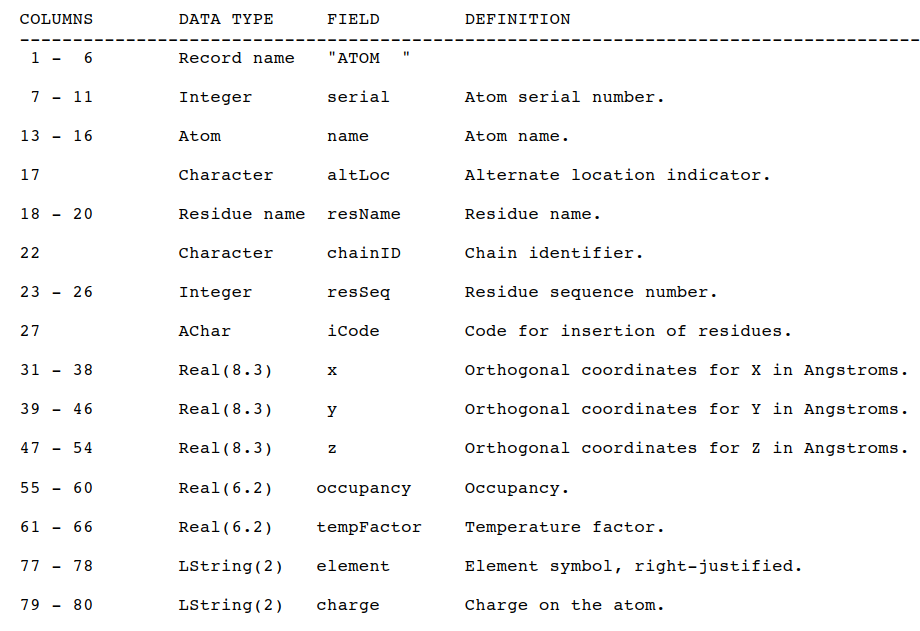
\includegraphics[width=\textwidth]{img/pdb.png}
\end{center}

CAST won't assign atomtypes to PDB structures but you can use the task \texttt{WRITE\_XYZ} to get an xyz-file. If you take this xyz-file as input atomtypes will be assigned. If there are several alternate locations for an atom only the first location (``A'') will be read in.


%%%% Fixations and biases %%%%
\subsection{Fixations, Biases and coordinate manipulations}
\ac{CAST} is able to work with bias potentials and atom fixation globally in all methods. Global optimization routines will usually operate on \textit{main dihedrals}. \textit{Main dihedrals} make up a subset of independent dihedrals. Rotating a main dihedral often implies the alteration of several dihedrals. \ac{CAST} uses a very generalized internal coordinate system which can be heavily tailored by expert users.

\subsubsection{Main dihedrals}

\begin{longtable}{|p{3cm}|p{5cm}|p{3cm}|}
	variable & effect & type [default value] \\
	\hline
	\textbf{REMOVEHROT} & Torsions involving hydrogen atoms will not be considered main torsions. & bool [true] \\	
	\textbf{MAINblacklist} & Black- or Whitelist a rotation around a bond for the selection as main rotation. & int, int [none] \\
	\textbf{MAINwhitelist} & Black- or Whitelist a rotation around a bond for the selection as main rotation. & int, int [none] \\
\end{longtable} 

\subsubsection{Fixations}

\begin{longtable}{|p{3cm}|p{5cm}|p{3cm}|}
	variable & effect & type [default value] \\
	\hline
	\textbf{FIXexclude} & Exclude nonbonded interactions between two fixed atoms when using force-field energy interfaces & int, int [none] \\
	\textbf{FIXrange} & Numbers of atoms that are fixed (indizes in tinker numbering, i.\,e. starting with 1) & int-range [none] \\
	\textbf{FIXsphere} & Define a sphere outside of which atoms are fixed. Sphere is defined by two numbers, first is the atom index of the atom that is at the center of the sphere& int double [none] \\
\end{longtable} 

\textbf{Attention!} Atom fixations do not work with AMBER input!

\subsubsection{Biases}

\begin{longtable}{|p{3cm}|p{5cm}|p{3cm}|}
	variable & effect & type [default value] \\
	\hline
	\textbf{BIASspherical} & Arbitrary Spherical Bias Potential centered at origin & radius force exponent [none] \\
	\textbf{BIAScubic} & Arbitrary Cubic Bias Potential centered at origin & x y z force exponent [none] \\
	\textbf{BIASdist} & Harmonic potential on an atom distance & atom1 atom2 distance force [none] \\
	\textbf{BIASdih} & Harmonic potential on an arbitrary dihedral angle & atom1 atom2 atom3 atom 4 angle force [none] \\
	\textbf{BIASangle} & Harmonic potential on an arbitrary angle & atom1 atom2 atom3 angle force [none]
\end{longtable} 

If you want to apply more than one bias of the same kind just repeat the keyword.

Furthermore it is also possible to apply a harmonic potential on a linear combination of atom distances. Because this kind of bias was first implemented in the umbrella sampling part of CAST you have to switch it on in the umbrella part of the CAST.txt inputfile by setting \texttt{USuse} to 1. Then you can define your potential by the keyword \texttt{UScomb} as described in section \ref{sec:umbrella}.
	
	
	%%%% TASKS %%%%
	\subsection{Tasks}
	The main computations in \ac{CAST} are called \textit{tasks}. They are invoked with the configuration file keyword \glqq\textit{task}\grqq~followed by the identifier of the desired computation. On the following pages outline the individual tasks that can be performed by \ac{CAST}.

	\newpage

	%%%%%%%%%%%%%%%%%%%%%%%%%%%%%%%%%%%%%%
	%%%%                              %%%%
	%%%%     Specific Tasks           %%%%
	%%%%                              %%%%
	%%%%%%%%%%%%%%%%%%%%%%%%%%%%%%%%%%%%%%
	\section{Specific Tasks}

	%%%% SP %%%%
	\subsection{SP - Single point energy calculation}
	A single point calculation calculates the potential energy of the respective system. Single point calculations can be run either using a force field or one of the external energy interfaces. In case of force field calculations the output is decomposed into the different force field contributions.\\

	The output consists of the abbreviations for the different force field contributions as well as their respective energy in $\frac{kcal}{mol}$. At the end the total potential energy is given in $\frac{kcal}{mol}$.\\~\\

	\begin{longtable}{l|l}
		symbol & energy\\
		\hline
		\textbf{B} & Bond energy\\
		\textbf{A} & Angle energy\\
		\textbf{U} & Urey-Bradley energy (\ac{CHARMM})\\
		\textbf{ID} & Improper dihedrals energy (\ac{AMBER}, \ac{CHARMM})\\
		\textbf{IT} & Improper torsions energy (\ac{OPLS-AA})\\
		\textbf{V} & Van-der-Waals energy\\
		\textbf{C} & Charge energy\\
		\textbf{SOLV} & Solvent energy (if implicit solvent is used)\\
		\textbf{SUM} & Total potential energy\\

	\end{longtable}


	%%%% GRAD %%%%
	\subsection{GRAD - Single point energy and gradient calculation}
	The result of a gradient calculation is the same as the result for a single point calculation with the addition that the gradients of the atoms are also calculated. The output can be found as a file where the filename specified by the configuration parameter "output" is amended by the keyword "GRAD". This file contains the information about the gradients with respect to atoms, force field contributions and x-, y- and z-coordinates. If an external interface is used only the total gradients in x-, y- and z-direction on every atom are given.
	
	\subsection{HESS - Single point energy and hessian calculation}
	The result of this task is also the same as for a single point calculation. In addition to the energy the hessian matrix is also calculated. You find the matrix in a file called \textit{outname}\_HESS.txt. Currently the calculation of hessians is only implemented in the DFTB\textsuperscript{+} and DFTBaby interface so it will give an error for other interfaces.
	

	%%%% LOCOPT %%%%
	\subsection{LOCOPT - Local optimization}
	\label{sec:locopt}
	\ac{CAST} is using the L-BFGS algorithm\supercite{bfgs} with the More and Thuente linesearch\supercite{morethuente} for local optimizations if an interface without optimizer is used or additional forces are applied. An example for this is using force fields as the energy interface.  \todo{what does additional forces applied mean?}
	If an interface with included optimizer (most external interfaces) is used (and if no bias forces are to be applied), the optimization process will be carried out by those programs and \ac{CAST} will only retrieve the final geometry and gradient values.
	The integrated L-BFGS can be adjusted regarding the maximum number of steps performed in the optimization routine via the "BFGSmaxstep"\ configuration option $($default "10000"$)$.
	The convergence criterion can be altered using "BFGSgrad" $($default "0.001"$)$.

	\begin{longtable}{|p{4cm}|p{5cm}|p{2cm}|}
		variable & effect & default \\
		\hline
		\textbf{BGFSgrad (float)} & Threshold for gradients & 0.0001 \\
		\textbf{BFGSmaxstep (integer)} & Number of max BFGS steps & 10000 \\
		\textbf{BFGStrace (bool)} & if on, intermediate structures are written into a file ``trace.arc'' \begin{itemize} \item 0 = off \item 1 = on\end{itemize} & false \\
	\end{longtable}

	%%%% MD %%%%
	\subsection{MD - Molecular Dynamics}
	The MD keyword is used to start a \acf{MD} Simulation\supercite{md_art}. \acp{MD} can be performed in NVE, NVT and NPT ensembles. For temperature control a Nose-Hoover thermostat\supercite{nose,hoover} is available or the temperature control can be done by direct velocity scaling. Pressure can be controlled by a Berendsen-barostat\supercite{berendsen}. If constant pressure is desired, the use of periodic boundary conditions is compulsory. Integration of the equations of motion can be done via Velocity-Verlet or Beeman\supercite{beeman} integration scheme (implementation see \cite{becker_development_2015}). 

	\begin{longtable}{|p{4cm}|p{4.5cm}|p{3cm}|}
		variable & effect & type [default value] \\
		\hline
		\textbf{MDsteps} & Number of MD steps & integer [10000] \\
		\textbf{MDintegrator} & Type of integrator \begin{itemize}
			\item 0  = Velocity-Verlet \item 1 = Beeman
			\end{itemize} 	
		& integer [0] \\
		\textbf{MDveloscale} & Remove translation and rotation at every step\begin{itemize} \item 0 = no \item 1 = yes\end{itemize}& integer [1] \\
		\textbf{MDtemp\_control} & Activate temperature control\begin{itemize} \item 0 = no \item 1 = yes\end{itemize}& bool [1] \\
		\textbf{MDthermostat} & Nosé-Hoover thermostat\begin{itemize} \item 0 = no \item 1 = yes\end{itemize} if yes, you have to define heatsteps by the option ``MDheat'', otherwise the results won't make sense & integer [0] \\
		\textbf{nosehoover\_Q} & Scalingfactor for Nose-Hoover Thermostat & double [0.1] \\
		\textbf{MDtimestep} & Timestep in picoseconds & float [0.001] \\
		\textbf{MDrestart\_if\_broken} & CAST tests after every MD step if all bonds are still intact. If this option is set to zero it just tells you (assuming the verbosity is high enough) which bonds are broken and the simulation continues. This will most probably lead to an explosion of your molecule and the breaking of the simulation. If this option is however set to 1 after recognising broken bonds the coordinates of all atoms are set to the original coordinates at the beginning of the simulation and new random velocities are assigned (according to the currently desired temperature, i.\,e. if you've applied a gradient the gradient won't start again but the temperature will continue to act how you would expect it if the simulation had run normally). This will prevent the simulation from breaking. & integer [0] \\
		\textbf{MDtrack} & Track MD and write output\begin{itemize} \item 0 = no \item 1 = yes\end{itemize}& integer [1] \\
		\textbf{MDtrackoffset} & Offset for tracked MD output (in frames, every \textit{n}'th frame will be written)& integer [1] \\
		\textbf{MDsnap} & Number of snapshots & integer [100] \\
		\textbf{MDsnap\_buffer} & Number of snapshots saved in memory before written to file & integer [50] \\
		\textbf{MDsnap\_opt} & Optimize snapshots with chosen energy interface\begin{itemize} \item 0 = no \item 1 = yes\end{itemize} & integer [0] \\
		\textbf{MDheat}  & Apply Heating \begin{itemize}\item1st value: snapshot number\item2nd value: temperature at snapshot\end{itemize} & none\\
		\textbf{MDpress} & Enable pressure control\begin{itemize} \item 0 = no \item 1 = yes\end{itemize}& integer [0]\\
		\textbf{MDpcompress} & isothermal compressibility in bar\textsuperscript{-1} & float [0.000046 (value for water)] \\ 
		\textbf{MDpdelay} & Barostat delay in picoseconds & float [2.0]\\
		\textbf{MDptarget} & Target pressure in atm & float [1.0] \\
		\textbf{MDspehrical} & Switches for spherical boundary conditions & integer, float, float, float, float, float, float [deactivated] (\textit{details below}) \\
		\textbf{MDrattle} & Switch for Rattle\supercite{rattle} H-bond constraints\begin{itemize} \item 0 = no \item 1 = all hydrogen bonds \item 2 = specific bonds (\textit{see below}) \end{itemize} & integer [0] \\
		\textbf{MDrattle\_use\_paramfile} & if true constrained distances are bond length parameters from the forcefield parameter file, if false the distance for every constrained atom pair must be given with the option MDrattledist & bool [true] \\
		\textbf{MDrattlebond} & Specify certain atom pairs for Rattle\supercite{rattle} if MDrattle = 2 (pairs of atom indices, starting with 1) & integer, integer [none] \\
		\textbf{MDrattledist} & distances to which the atom pairs given in MDrattlebond are constrained if MDrattle\_use\_paramfile is false. The rattlebonds and rattledists have to be given in the same order. If you use this option you can also constrain distances between non-bound atoms. & double [none] \\
		\textbf{MDbiased\_potential} & Switch on and off a biased potential around the active site \begin{itemize} \item 0 = off \item 1  = on \end{itemize} & integer [0] \\
		\textbf{MDactive\_site} & atom numbers of active site (write a new line for every atom) & integer [none] \\
		\textbf{MDcutoff} & inner and outer cutoff for biased potential & integer, integers [not defined] \\
		\textbf{MDadjust\_by\_step} & calculate the geometrical center for the active site and the distances to it new for every step \begin{itemize} \item 0 = no \item 1  = yes \end{itemize} & integer [not defined] \\
		\textbf{MDrestart\_offset} & Offset for restart file writing in frames & integer [0] \\
		\textbf{MDrefine\_offset} & Offset for nonbonded list generation, i.\,e. the list of non-bonded pairs is generated after the number of steps that is given here (useful if a cutoff radius for non-bonded interactions is given) & integer [0]  \\
		\textbf{MDresume} & Boolean switch for using a restart file to start MD\begin{itemize} \item 0 = no \item 1 = yes\end{itemize}& integer [0] \\
		\textbf{MDpre\_optimze} & Perform Optimization before starting the Simulation \begin{itemize} \item 0 = no \item 1 = yes\end{itemize}& integer [0] \\
			\end{longtable} 
	
	Note: In case you enable logging, the verbosity will be controlled by global verbosity setting.\\
	
	\ac{MD} Simulations use the common types of boundary conditions present in \ac{CAST}. For more information on this, see section \ref{sec:boundary}.

	\subsubsection{Heating}
	Note: The settings for "MDheat" can be applied multiple times. The first number indicates the snapshot number, the second one the desired temperature at this snapshot. If the "MDheat" keyword is specified multiple times heating and cooling can be applied sequentially during a single simulation. \ac{CAST} reads the "MDheat" keywords from top to bottom and starts with the first one, finishing with the one on the bottom.\\~\\
	\begin{lstlisting}
	MDheat			    0  	  0.0
	MDheat 			 1000   300.0
	MDheat			 5000   300.0
	MDheat			10000     0.0
	\end{lstlisting}~\\~\\
	In the above example the simulation starts at 0 Kelvin and is then heated to 300K within the first 1000 steps. The temperature is kept steady for 4000 steps until step 5000 is reached. Now the system is cooled back to 0 Kelvin during steps 5000 to 10000. The user has to take care that enough total steps are performed for the temperature scaling sequence!\\
	
	There are two possible ways for temperature control in CAST (for both of them MDtemp\_control has to be activated!): 

If you disable the option ``MDthermostat'' a simple velocity scaling is used for heating up. After reaching the desired temperature the control mechanism will keep the temperature constant. Setting the start temperature to zero will result in an error because there's a division by zero. So your settings for first heating up and then keeping the temperature constant (after 1000 steps) might be:
	\begin{lstlisting}
	MDheat			    0  	  0.0001
	MDheat 			 1000     300
	\end{lstlisting}

	The other possibility is the Nosé-Hoover thermostat that is used if ``MDthermostat'' is enabled. Then the Nosé-Hoover thermostat controls the temperature set by ``MDheat''. If you have switched on the thermostat you may set the starting temperature to zero. So if you want the same temperature evolution as above with the thermostat your input might be:
		\begin{lstlisting}
	MDheat			    0  	  0
	MDheat 			 1000     300
	\end{lstlisting}
	
	For details about the Nosé-Hoover thermostat, especially the factor(s) Q which you can set in CAST, see \cite{frenkel_understanding_2001}.
	
\textbf{	Running an MD without temperature contol}
	
	\ac{CAST} can also be run without temperature control. One option to do this is just to set MDthermostat to 0 and delete all lines starting with MDheat. Then the simulation starts at 0\,K and no thermostat is applied during the run so the total energy is kept constant. If you don't want to start the simulation at 0\,K you can set MDtemp\_control to 0. Then every kind of temperature control is also switched off but you can set a starting temperature different from 0\,K. To do so use the option MDheat. The starting temperature is always the first temperature that you set with that option, no matter which step you set. So if you write this:
			\begin{lstlisting}
	MDheat			  200  	  50
	MDheat 			 1000     300
	\end{lstlisting}
	the starting temperature (at step 0) is 50\,K and the second line is just ignored. To avoid confusion it is recommended only to use one line of MDheat and set it to step 0:
\begin{lstlisting}
MDheat			    0  	  300
\end{lstlisting}	

\subsubsection{Rattle}

You can use the Rattle Algorithm\supercite{rattle} to constrain atom distances during the MD simulation. With the option ``MDrattle'' you activate this option. If it's set to 1 all bonds that contain a hydrogen atom are automatically constrained, if it's set to 2 you can choose atom pairs to constrain. Another important option for rattle is ``MDrattle\_use\_paramfile''. If it's set to true (default) the distances to which the atom pairs are constrained are taken from the forcefield parameter file. If you use MDrattle=1 you have to use this option. If some of your atom pairs don't share a bond you can't use this option because it wouldn't make sense to constrain them to the bond distance. 

If you want to define the atom pairs to be constrained yourself you do that with the option ``MDrattlebond''. There you give the atom indices (starting with 1) of your atom pairs. Every atom pair is in a new line so this section might look like this:
\begin{lstlisting}
MDrattlebond           3117   347
MDrattlebond           3160   2276
\end{lstlisting}

If you have chosen not to use the bond distances from the parameter file but to define your own atom distances you use the option ``MDrattledist''. There you give the atom distances for the atom pairs defined in ``MDrattlebond''. Again every atom pair gets its own line. So if you want to constrain the distance between atoms 3117 and 347 to 2.5\,\AA~and that beween atoms 3160 and 2276 to 1.1\,\AA~this section is:
\begin{lstlisting}
MDrattledist           2.5
MDrattledist           1.1
\end{lstlisting}
		
	\subsubsection{MD with biased potential}
	
	By setting the option ``MDbiased\_potential'' from 0 to 1 you can switch on a biased potential. This means that the movement of the atoms depends on the distance of every atom to the active site that is defined by the option ``MDactive\_site''. Atoms near the active site move ``normally'' whereas the speed of atoms with a larger distance to the active site is scaled down until there's no movement. With the option ``MDcutoff'' you can modify the strength of the biased potential. The first number is the distance around the active site where no additional potential is applied, the second number is the distance around the active site outside of which there's no movement. During the MD the distances of the atoms to the active site change. If you want to take this into account set the option ``MDadjust\_by\_step'' to 1. Then the position of the active site as well as the distances are calculated new for every step. If ``MDadjust\_by\_step'' is set to 0 the position of the active site and the distances are calculated only once and stay constant for every atom during the simulation. 
	
If an FEP calculation is done you can set the ``MDactive\_site'' to zero instead of atom numbers. Then the active site is defined by all atoms that appear or disappear during the reaction, e.\,g. that are marked by ``IN'' or ``OUT'' in the coordinate file. 
	
If you use the ``MDheat'' option the temperature (and thus the scaling factor) is only calculated by the velocities for the atoms inside the inner cutoff radius where the movement is not manipulated. The kinetic energy is however calculated for all atoms so they do not fit together directly. 

Don't use ``MDveloscale'' with biased potential because it doesn't make sense to rotate the whole molecule if only a part of it moves during the simulation.

\subsubsection{Tools to analyze MD simulations}

You can perform several graphical analyses on MD trajectories. To create the graphs CAST uses the python matplotlib module so you have to compile CAST with python enabled and matplotlib must be installed. If you don't have python enabled you get a warning that plotting is not possible without python. The information you need for the MDanalyze\_zones option is nevertheless saved in the outputfile ``zones.csv'' and the distances for atom pairs in ``distances.csv''.

By the option ``MDana\_pair'' you can choose one or more atom pairs whose distances are plotted during an MD simulation into an image called ``distances.png''. The two atoms of the atom pair are seperated by a comma. For analyzing more than one atom pair just repeat the option several times. So this section might look: 
			\begin{lstlisting}
MDana_pair         347,3149
MDana_pair         2277,3151
MDana_pair         2277,2276
	\end{lstlisting}
	You get the same picture if you run the script ``plot\_MD\_distances.py'' over the CAST outputfile ``*\_MD\_SNAP.arc'' if you have saved a snapshot of every step.

Another possibility is ``MDanalyze\_zones''. If you activate this option CAST first determines zones around your active site (defined by ``MDactive\_site'', geometrical center of those atoms) with the width ``MDzone\_width''. For each of those zones CAST saves the average temperature after every step and plots them after the simulation into the file ``zones.png''. 
	
%%%% GOSOL %%%%
\subsection{GOSOL - Global Optimization and Solvation}	
 \todo[inline]{write something about task GOSOL} 

	
	%%%% Global Optimization (GO) %%%%
	\subsection{TS, MC - Global Optimization Tasks}
	\ac{CAST} can be used to perform Conformational Analysis. To find the lowest possible conformation, either a standard Monte-Carlo-Simulation\supercite{mc_original, mmc_original} or a Tabu-Search\cite{tabusearch_original1, tabusearch_original2, tabusearch_original3} based approach can be choosen. The total number of steps for the global optimization routines is set by ``Iterations'' (default ``1000''). \ac{CAST} will save all minima between $E_0$ (current lowest energy) and $E_0 + D$ where the value of D is adjusted with the ``Erange'' keyword (default ``0.0'').
	If the current step does not result in a newly accepted minimum, \ac{CAST} will select a new starting point. The key ``GOfallback'' selects either a simple fallback to local / global minimum (value ``LAST\_GLOBAL'', default) or an evolutionary selection algorithm (value ``EVOLUTION'').
	
	\begin{longtable}{l|l|l}
	variable & effect & default \\
	\hline
	\textbf{Iterations} & Number of iterations & 1000 \\
	\textbf{Erange} & Energy range for output & 0.0 \\
		\textbf{GOfallback} & Type of fallback & LAST\_GLOBAL \\
	\end{longtable}
	
	%% Starting point selection
	\subsubsection{Starting point selection}
	\textbf{Simple Fallback} \\
	This method uses the parameter ``GOfallback\_limit'' to determine how often the program can use a specific minimum as a starting point. If the limit for the last accepted minimum is reached, \ac{CAST} uses the current ``global'' minimum instead. If the limit for this minimum has also been reached, \ac{CAST} stops.\\
		
	%% Evolutionary selection
	\textbf{Evolutionary selection} \\
	This algorithm selects a new starting point among a limited number of minima N (the limit is set via ``GOincluded\_minima'' and defaults to 10.)
	A roulette selection algorithm is applied where the fitness of the respective structures is determined based on their energetic rank. A lower L and an upper bound H for the fitness can be specified using ``GOfitness\_bounds'' (default ``0.5 1.0'') where minimum N has fitness L and minimum 1 has fitness H.
	The interpolation between those points (1,H) -> (N,L) can be controlled by ``GOfitness'' where the value ``LINEAR'' (default) denotes linear interpolation while ``EXPONENTIAL'' activates exponential decay.
	\ac{CAST} makes up to 100 attempts to select a minimum which hasn't reached the limit yet and stops if none is found.
	
	\begin{longtable}{|p{3.5cm}|p{5cm}|p{2.5cm}|}
	variable & effect & default \\
		\hline
		\textbf{GOfallback\_limit} & Number of times a minimum can be used & - \\
		\textbf{GOincluded\_minima} & Number of minima to look for new starting point & 10 \\
		\textbf{GOfitness\_bounds} (2 values) & Lower and upper bound for fitness & 0.5 1.0 \\
		\textbf{GOfitness} & Interpolation between \textbf{GOfitness\_bounds} & LINEAR \\
	\end{longtable}

	%% Metropolis Criterion
	\textbf{Metropolix Criterion} \\
	The global optimization routines in \ac{CAST} evaluate the energy of a certain conformation (E) using the Metropolis criterion (MEC).
	\begin{equation}
	R < e^{-\frac{E-E_0}{kT}}
	\end{equation}
	\\~\\
	with R: Random number ($0 <= R <= 1$)
	and E: Evaluated energy
	and $E_0$: Reference energy
	and k: Boltzmann constant
	and T: Temperature\\~\\
	
	The reference energy E\_0 can either be the energy representing the most stable structure (current ``global minimum'') or the last local minimum energy. The corresponding control option is called ``GOmetrolocal'' and defaults to 0 (off) which means that the current global minimum energy is used in the conditional. A value of ``1'' will make \ac{CAST} use the ``current local minimum'' energy (the starting point of the current iteration). If the Metropolis Criterion is not met, the conformation will be discarded.
	The temperature used is controlled via ``Temperature'' and defaults to ``298.15''. It is multiplied by a factor, adjusted via ``Tempscale'' (default: ``1.0'').\\~\\
	
	\begin{longtable}{|p{3.5cm}|p{5cm}|p{2.5cm}|}
		variable & effect & default\\
		\hline
		\textbf{GOmetrolocal} & Use global or current local minimum energy as reference; 0 = no, yes = 1 & 0 \\
		\textbf{Temperature} & Temperature in Kelvin & 298.15 \\
		\textbf{Tempscale} & Multiplication factor for temperature & 1.0
	\end{longtable}
	
	%% Monte Carlo
	\subsubsection{MC - Monte Carlo}
	The \ac{MC} simulation will move the system randomly across the \ac{PES} and evaluate the reached point either directly or after local optimization. The ``MCminimization'' option turns minimization on (value ``1''; default) or off (value ``0''). 
	
	\textbf{Attention!}
	If you use an energy interface that doesn't work with bonding information when calculating the energy it is possible that you get a minimum structure that looks very strange to you. For an example see figure \ref{fig:dist_eth} which is an ethanole molecule. This is not a bug because if you rebind the atoms by a distance criterion everything will be fine again. The atoms are just shuffled around randomly and then the energy is evaluated out of the atom positions. So it doesn't matter to the program if for example two hydrogen atoms have swapped positions. One possibility to avoid this is to use the move type ``main dihedral'' instead of ``cartesian''. Another possibility is to turn on preoptimization with a force field as energy interface.
	
		\begin{figure}[htb]
		\centering
		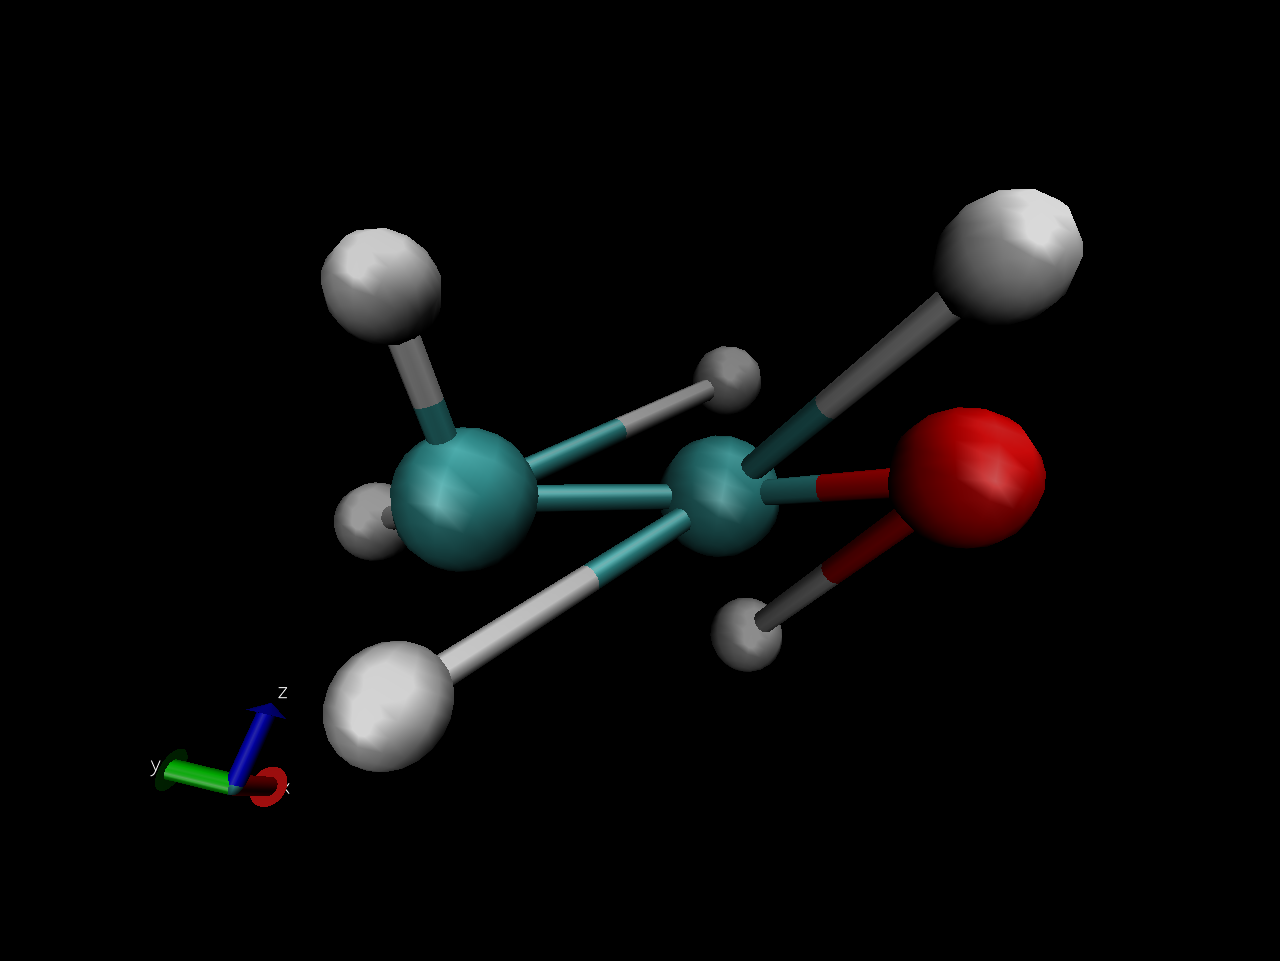
\includegraphics[width=0.5\textwidth]{img/distorted_ethanol.png}
		\caption{Ethanole molecule that is distorted by MC calculation}
		\label{fig:dist_eth}
	\end{figure}
	
	\textbf{Move types}\\~\\
	\ac{CAST} can move to the next sampling point during \ac{MC} in three different ways, controlled via the ``MCmovetype'' option (default ``1''). A value of ``2'' will make the program carry out the contortion in Cartesian space (where the ``MCstep\_size'' option with a default value of ``2.0'' will restrict the absolute value of the distortion vector). The value ``1'' represents direct rotation of randomly selected main dihedral angles (see 1.5). A value of ``0'' means that the target conformation is not obtained directly by adjusting dihedrals but the conformational change will be achieved by applying quadratic bias potentials on the main dihedrals towards the target conformation during a local optimization process (``MCmax\_dihedral'' restricts the maximum distortion of a dihedral angle; default ``160.0''). \\
		
	\begin{longtable}{|p{3cm}|p{5cm}|p{3cm}|}
		MCmovetype value & Move type & Associated options \\
		\hline
		0 & Biased main dihedral optimization & MCmax\_dihedral \\
		1 & Main dihedral & MCmax\_dihedral \\
		2 & Cartesian & MCstep\_size \\
	\end{longtable}

	The number of distorted dihedrals is selected randomly in case of a ``MCmovetype'' value of 0 or 1 (biased or direct main dihedral adjustment).
	\begin{equation}
	N = - log (R) + 1
	\end{equation}
	with R being a random number between 0 and 1 and N being the number of distorted rotated dihedrals.\\~\\
	\begin{longtable}{|p{3.5cm}|p{5cm}|p{2.5cm}|}
		variable & effect & default \\
		\hline
		MCminimization & Turn minimization on or off; 0 = off, 1 = on & 1 \\
		MCmovetype & Movetype to go to next sampling point & 1 \\
		MCstep\_size & Absolute value of distortion vector & 2.0 \\
		MCmax\_dihedral & Maximum distortion of dihedral angle in degre & 160.0 \\
	\end{longtable}
		
	%% Tabu Search
	\subsubsection{TS - Tabu Search}
	The \acf{TS} process in \ac{CAST} is essentially an alternating combination of the dimer method\cite{dimermethod} and the local optimization process (see section \ref{sec:locopt}).
	If a certain number of \ac{TS} iterations do not yield a new and acceptable minimum, the \acf{DS} process (\ac{MC} with minimization is used here) is executed. The option controlling how many steps need to fail before diversification search comes into place is called ``TSdivers\_threshold'' (default ``25'').
	The ``TSdivers\_iter'' option (default ``30'') represents the number of iterations during one diversification routine.
	If you want \ac{CAST} to start with \ac{DS} iterations instead of the \ac{TS} iteration you can set ``TSmc\_first'' to ``1'' (default ``0'').\\~\\
	
	\begin{longtable}{|p{3.5cm}|p{5cm}|p{2.5cm}|}
		variable & effect & default \\
		\hline
		TSdivers\_threshold & Number of failed steps before \acl{DS} & 25 \\
		TSdivers\_iter & Number of iterations during diversification & 30 \\
		TSmc\_first & Start with diversification instead of Tabu-Search iterations; 0 = no, 1 = yes & 1 \\
	\end{longtable}

		%% Output
	\subsubsection{Output}
	The output for verbsity settings of 2 and higher includes 15 columns (with \textit{NA} being the number of currently accepted minima):\\
	\begin{itemize}
		\item Method (\ac{MC}, \ac{MCM} or \ac{TS})
		\item Current iteration
		\item \todo{I guess that means blank line, does it?} 
		\item Maximum number of iteration
		\item Index of current minimum in the interval (0, \textit{NA})
		\item Current minimum energy (starting point of current step)
		\item "Transition step" energy (energy after distortion / dimer method without optimization)
		\item New minimum energy (after optimizing the "transition step" structure).
		\item Identifier for acceptance (A = accepted; R = rejected)
		\item Acceptance information
		\begin{itemize}
			\item ok = new minimum, but not lowest
			\item GM = new minimum, lowest
			\item energy = rejected because of metropolis criterion
			\item broken = Configurational feature of the structure broken
			\item tabu = already visited minimum
		\end{itemize}
		\item Number of accepted minima (\textit{NA})
		\item Number of minima within the energy range
		\item Current temperature used for the metropolis criterion
		\item Iteration Runtime
		\item Number of CPU clock ticks required for current iteration
	\end{itemize}
	
	Example:\\
	\begin{lstlisting}
	MCM; 87/100; 0 -2.0604e+02; -1.8566e+02; -2.0516e02;
	R (energy) 1 1 (47.04 K, 3.37s (33701 ticks))
	\end{lstlisting}

		%%%% Dimer Method (DIMER) %%%%
	\subsection{DIMER - Dimer Method}
	This task will perform the improved dimer-method for finding transition states\supercite{dimermethod}. The "dimer size" (magnitude of dimer vector) can be controlled via "DIMERdistance" (default "0.01").
	It is possible to adjust the maximum rotational force during the dimer translation. The dimer translation is interrupted and the dimer is rotated into the minimum in case this limit is exceeded. The key controlling this value is called "DIMERtflimit".
	The maximum number of iterations for the dimer rotation and translation steps can be set in the combined "DIMERmaxit" option, which takes two parameters where the first one limits the number of rotation iterations per translation step while the second one represents the maximum number of translations.
	The convergence criterion for the dimer rotation (the angle that needs to be undercut) in degrees can be adjusted using "DIMERrotconvergence".
		
	\begin{longtable}{|p{4cm}|p{3.5cm}|p{2.5cm}|}
		variable & effect & default \\
		\hline
		\textbf{DIMERdistance} & Controls magnitude of dimer vector & float [0.01] \\
		\textbf{DIMERtflimit} & Controls magnitude of dimer force & float [0.01] \\
		\textbf{DIMERmaxit}& Controls rotation steps per translation and total translation steps & integer, integer [20 100]\\
		\textbf{DIMERrotconvergence} & Convergence criterium for rotation in degree & float [5.0] \\
	\end{longtable}
	
	%%%% UMBRELLA %%%%
	\subsection{UMBRELLA - Umbrella Sampling} \label{sec:umbrella}
	The \acf{US}\supercite{umbrellasampling1, umbrellasampling2, umbrellasamplingreview} implementation features four kinds of reaction coordinates which can be sampled: distances, angles, dihedral angles or linear combinations of distances. Distances can be chosen between any two particles in the system, angles between any three of them. Dihedrals can be defined between any four particles in the system. None of the reaction coordinates is limited to existing internal coordinates of the system.
	The \acl{US} implementation is divided into two parts: equilibration with the applied bias potential and a production run with the applied bias potential. For all reaction coordinates a half harmonic potential is used. The number of steps for equilibration is defined by the \glqq\textit{USequil}\grqq~configuration variable. The number of production steps is defined by the \glqq\textit{MDsteps}\grqq~variable.

	\begin{longtable}{|p{3cm}|p{5cm}|p{3cm}|}
		variable & effect & default \\
		\hline
		\textbf{USequil} & number of equilibration steps & integer [0] \\
		\textbf{USsnap} & Offset for snapshots (Snapshot every x steps) & integer [0]  \\
		\textbf{UStorsion} & Definition for torsion angle & integer, integer, integer, integer, float, float [none] \\
		\textbf{USangle} & Definition for angle & integer, integer, integer, float, float [none] \\
		\textbf{USdist} & Definition for distance & integer, integer, float, float [none] \\
		\textbf{UScomb} & Definition for combination of distances & [none] \\
	\end{longtable}

	The syntax for the definition of the restraints can be seen in the following listing:\\
    
	\begin{lstlisting}
	#Torsion: <atom 1> <atom 2> <atom 3> <atom 4> <force> <value>
	UStorsion       1        5        7        9    0.05    0.0
	
	#Angle            <atom 1> <atom 2> <atom 3> <force> <value>
	USangle             2          1        3    1000.0   90.00  
	
	#Distance: <atom 1> <atom 2> <force> <value>
	USdist           1        9    10.0    3.0
	
	# Combination of distances:
	# <number of dist> <force> <value> ( <index1> <index2> <factor> ) 
	# for every distance: another ( <index1> <index2> <factor> ) 
	UScomb          2      50   -1.9   ( 1  2  +1 ) (  1  6  -1 )
	\end{lstlisting}
	~\\
	Torsion restraints consist of 6 values: the first 4 integers are the index numbers of the atoms which form the dihedral. Indices start at "1". The fifth number is the force constant of the harmonic potential in $\frac{kcal}{mol \cdot deg^2}$ and the last index the desired value of the angle in degrees.
	
	An angle restraint consists of the 4 atom indizes (second one is the peak of the angle), the force constant in $\frac{kcal}{mol \cdot deg^2}$ and the desired value in degrees.
	
	The distance restraint consist of the two indices for the atoms, the force constant in $\frac{kcal}{mol \cdot {\mathring{A}}^2}$ and the distance in \AA.

	
	If you want to define your reaction coordinate as a linear combination of distances, i.\,e. $\xi = \sum_j f_j \cdot d_j$ with scaling factor $f_j$ and distance $d_j$ you first have to give the number of distances you want to include into your reaction coordinate, then the force in $\frac{kcal}{{\mathring{A}}^2}$ and then the value to which it is restrained. After that you have brackets for every distance you include. Inside the brackets are the indices of the atoms that form the distance and the scaling factor. In the example above the reaction coordinate is $\xi = d_{12} - d_{16}$. It is important that there is a space before and after every bracket.
	
	\textbf{Attention!} If you use bonds as reaction coordinates you should start the simulation with a structure where the reaction coordinate is similar to the restraint. Otherwise you will in best case get a lot of warnings about broken bonds and in other cases the simulation will break because of too much energy. This in principle also applies to combinations of bonds but there the force constant slowly rises during the first half of equilibration so the forces in the beginning aren't that big and the system can gradually adapt to the restraint. If you want this behaviour with a distance as reaction coordinate you can also define a combination of just one distance.
	The \acl{US} output is written to a file named ``umbrella.txt''. For every window one has to start an individual run with the corresponding value of the restraint. The output is formatted for use with the \ac{WHAM} program\supercite{wham1, wham2} for post-processing. For details on the use of WHAM we refer the reader to the corresponding \ac{WHAM} manual.
	
	In our tutorial we describe in detail how to perform an Umbrella Sampling including the analsis with WHAM.
	
	\textbf{2D Umbrella}
	
	It is also possible to perform umbrella sampling in two dimensions. An example how to perform such a simulation is also described in detail in the tutorial. Some python scripts help you to perform and analyse the simulation. Those steps are recommended:
	
	\begin{itemize}
		\item Start MD simulations either with \texttt{fake\_queue\_umbrella2D.py} (for longer calculations) or with \texttt{fake\_queue.py} which calls \texttt{python.sh} and \texttt{umbrella2d\_helper.py} (for short calculations)
		\item Start WHAM with \texttt{umbrella2d\_analysis.py}
		\item Plot distributions and check if all simulations are okey with \texttt{umbrella2d\_check.py}
		\item Plot heatmaps for Free Energy and Probability with \texttt{umbrella2d\_plot.py}. This script also writes a csv file which can be used as input for \texttt{walkThroughSurface.py} which finds lowest energy path through the surface or for \texttt{walkOnPath.py} which walks through the surface on a given path.
		\item If desired: create more detailed plots with \texttt{umbrella2d\_cut.py} and \texttt{umbrella2d\_add.py}
	\end{itemize}

    If you don't want the whole free energy surface but just a given path you don't have to perform MDs on every point of the surface but only on those on or near the path. An example of that is also described in the tutorial.

	%%%% NEB %%%%
	\subsection{NEB - Nudged Elastic Band Method}	
NEB is a double ended or chain of states method in which the start and the end position has to be known in order to generate a reaction path. 
The following NEB methods are included in the CAST program: Standard method Henkelman and Jonsson\supercite{JonssonH.1998}, improved tangent estimate\supercite{Henkelman2000}, climbing image variant\supercite{Henkelman2000a}, temperature dependent neb\supercite{Crehuet2003} and image dependent pair potential for improved interpolation\supercite{Smidstrup2014}.
In the following the procedure how to do a NEB calculation should be illustrated on the example of the rotation of pentane.\newline

\begin{itemize}
	\item 
	\textbf{First steps}\newline
	The first step is the preparation of the Input structures. For exclusion of translational and rotational
	degrees of freedom the structures should aligned beforehand. This can be done by using the \texttt{TASK ALIGN} in CAST or e.g. VMD for this purpose. It is also important that the ordering of atoms is identical in both structures which are used.
	The first structure is defined as the standard input structure by using  the keyword \texttt{name} (-name=input1.arc). The second structure is defined by the keyword \texttt{NEB-PATHOPT-FINAL}. For all methods applying an optimization via the NEB scheme the
	following keywords have to be assigned:
	
	\texttt{NEB-PATHOPT-IMAGES} \textit{integer value} - defines the total number of interpolated structures which define the band\newline
	
	\texttt{NEB-PATHOPT-SPRING} \textit{floating point value} - defines the strength of the force which couples the structures of the band and is defined in kcal/mol$\AA^{2}$  \newline
		
	
	\item \textbf{Standard NEB method}
	
	In NEB the band is defined by $N+1$ structures $\{ R_{0},R_{1},...,R_{N} \}$. The start ($R_{0}$) and the final structure ($R_{N}$) remain unchanged by the optimization process. They serve as the anchor points of the band. The force which acts on a projected structure is the sum of the perpendicular component with respect to the derivative of the potential energy function $\nabla E(R^{\bot}_{i})$ and the tangential component $F^{||}_{i}$. In this way the force $F_{i}$ on the projected structure is
	
	\begin{equation}
	F_{i}=F^{||}_{i}-\nabla E(R^{\bot}_{i}),
	\end{equation}
	thereby one can write the resulting force (derived from the potential energy function) as:
	
	\begin{equation}
	\nabla E(R^{\bot}_{i})=\nabla E(R_{i}) -\nabla E(R_{i})\cdot \hat{\tau}_{i}.
	\end{equation}
	Within these equations $E$ describes the potential energy of the system which is a function of the atomic coordinates. The normalized tangent vector is denoted by $\hat{\tau}_{i}$, whereas $i$ stands for the projected structure although the calculation is atom wise defined. The force component along the band (tangential) is the spring force and defined as
	
	\begin{equation}
	F^{||}_{i}=k\left(\left|R_{i+1}-R_{i}\right|-\left|R_{i}-R_{i-1}\right|\right)\hat{\tau}_{i},
	\end{equation}
	with $k$ the spring constant. The modified force is then used by the optimizer to find the relaxed pathway. 
	
	\begin{itemize}
		
		\item \texttt{NEB-PATHOPT-TAU} is set to 0 using the standard tangent approach 
		
	\end{itemize}
	
	
	\item \textbf{Climbing image and improved tangent estimate}
	
	Various improvements of the standard NEB approach exist. One example is the climbing image (CI) variant which is only a small correction with respect to the standard approach. The information about the MEP is included as well, as the better convergence to the TS. Within the CI calculation the maximum energy image is calculated within the optimization procedure, whereas the calculation is repeated for each step. This projected structure is then called $i(MAX)$. For this special structure the force acting on it is computed in a modified approach:
	
	\begin{equation}
	F_{i(MAX)}=-\nabla E(R_{i(MAX)})+2 \nabla E(R^{||}_{i(MAX)}).
	\end{equation}
	In detail this equation can be written as:
	\begin{equation}
	F_{i(MAX)}=-\nabla E(R_{i(MAX)})+2\nabla E(R_{i(MAX)})\cdot \hat{\tau}_{i((MAX)}\hat{\tau}_{i((MAX)}.
	\end{equation}
	Within the CI variant the maximum energy structure is not influenced by the spring forces during the optimization step. 
	
	\begin{itemize}
		
		\item \texttt{NEB-PATHOPT-CI} \textit{bool value} - is set to 1 to use the climbing image variant.
		
	\end{itemize}
	
	Within the improved tangent estimate the connecting vectors $\tau$ are defined in the following manner:
	
	\begin{equation}
	\tau_{i}=\frac{R_{i}-R_{i-1}}{\left|R_{i}-R_{i-1}\right|}+\frac{R_{i+1}-R_{i}}{\left|R_{i+1}-R_{i}\right|}.
	\end{equation}
	
	\begin{itemize}
		
		\item \texttt{NEB-PATHOPT-TAU} \textit{bool value} - is set to 1 using the improved tangent approach.
		
	\end{itemize}
	
	
	
	\item \textbf{Temperature dependent NEB (MAXFLUX)}
	
	The temperature dependent NEB method accordingly to Crehuet and Field  is based on the maximization of the flux related to the Smoluchowski equation\supercite{Smoluchowski1916}. The method applies a differential equation and is directly inherited within the NEB algorithm. Starting from the Smoluchowski equation, Berkowitz and co-workers\supercite{Berkowitz1983} showed how the flux j of an optimal reaction path P can be expressed
	
	\begin{equation}
	j_{p} = \frac{const}{y\int_{p}exp(\beta U)ds},
	\label{eq:flux1}
	\end{equation}
	whereas along an ideal pathway (which is assumed to exist) all particles will flow and the friction $y$ is constant for all positions. Hereby $U$ is the potential energy and $s$ the position of the particles along the path. The factor $\beta$ is equal to $ 1/k_{b}T$. One way to optimize the flux is the discretization of the integral, $ \int_{p} exp(\beta U)ds$ given in Equation \ref{eq:flux1}. This can be done using the Euler formalism leading to the function $F$:
	\begin{equation}
	F(R_{1}...R_{N})=\sum^{N-1}_{i=0}\frac{1}{2}(e^{(\beta U (R_{i+1}))} + e^{(\beta U (R_{i}))})\left|R_{i-1}-R_{i}\right|.
	\end{equation}
	Within this equation, $ R_{i} $ is the coordinates vector of the i-th image along the pathways. $N$ is the total number of images/configurations. Starting from the discrete function, also gradients can be derived numerically. Still instabilities may arise during the optimization due to the presence of the exponential terms. Crehuet and Field\supercite{Crehuet2003} present a different approach to circumvent this issue. They start with the differential equation related to the Euler-Lagrange equation for the above mentioned integral (see Equation \ref{eq:flux1}). Therefore, one obtains the equation of Berkowitz and co-workers in the following form:		
	\begin{equation}
	\kappa \hat{t} + \hat{n} (\nabla \beta U \cdot \hat{t})-\nabla \beta U = 0.	
	\end{equation}
	Within this equation, the gradient along the reaction pathway is defined as $ g = \nabla U$ and the curvature of the RP is $\kappa$. The tangent and the normal vectors are $\hat{t}$ and $\hat{n}$. In a next step one can split the gradient into its components along and perpendicular to the band $ g = g_{||} + g_{\bot} $. The perpendicular component can be described as follows:	
	\begin{equation}
	g_{\bot}=\frac{\kappa}{\beta} \hat{n}.
	\end{equation}
	Using this equation, the transition between steepest descent pathways and finite temperature pathways is obtained. For $T\rightarrow 0K$ the equation is equal to $ g_{\bot}=0$. At infinite temperatures the path is straight, because all existing barriers can be overcome. Also $\kappa$ must be zero, as $ \beta \rightarrow 0$ and $g_{\bot}$ is not allowed to be singular. This new scheme for the perpendicular gradient component can be easily applied to the existing NEB scheme using the projection scheme. The force component which defines the perpendicular acting part of the NEB forces can be redefined,
	\begin{equation}
	F^{\bot}_{i}=g^{\bot}_{i} - \frac{\kappa}{\beta} \hat{n}
	\end{equation}
	whereas the force acting on the i-th atom is shown. The curvature of the band is defined by,	
	\begin{equation}
	\kappa_{i}=\frac{arccos(\hat{\tau}_{i-1}\cdot\hat{\tau}_{i+1})}{\left|R_{i}-R_{i-1}\right|+\left|R_{i+1}-R_{i}\right|}
	\end{equation}
	with $\tau_{i}$ the tangential vector along the band. The temperature dependent calculation is carried out by inclusion of the following flag:
	
	\item \texttt{NEB-PATHOPT-MAXFLUX}  \textit{bool value} - setting the value to 1 enable the temperature dependent calculation \newline
	
	Besides this flag also the temperature values have to be assigned using the specific flag. \newline
	
	\item \texttt{NEB-PATHOPT-TEMP} \textit{floating point value} - assigns temperature value in K
	
	
	
	
	\item \textbf{IDPP} 
	
	One of the first steps within a NEB calculation is the generation of the initial pathway which is built up by $N-2$ intermediate projected structures. Normally, this initial band is built up using a linear interpolation between the two starting minimum structures. Within this approach the interpolated structures can be far from being reasonable in terms of the internal coordinates (bonds, angles and dihedrals). Therefore, Smidstrup et al.\supercite{Smidstrup2014} introduced a new method for the calculation of the initial band of projected structures. This method is based on the interpolation of pairwise distances which are calculated for the whole band and additional acting forces which are deduced from these distances. The linearly projected structures ($R_{i}$) can be defined via their position vector ($r$), whereas each structure is built up by $N$ atoms. By using $i-2$ projected structures and the $start$ and $end$ structure, the interpolated distances between atom $n$ and $m$ at structure $i$	are given as
	\begin{equation}
	\begin{aligned}
	d^{i}_{nm} &= d^{start}_{nm} + \frac{i\left(d^{end}_{nm}-d^{start}_{nm}\right)}{N},\\
	&=\sqrt{\sum_{\sigma}\left(r_{n}-r_{m}\right)^2}\\
	&+\frac{i}{N}\left(\sqrt{\sum_{\sigma}\left(r_{n}-r_{m}\right)^2}^{end}-\sqrt{\sum_{\sigma}\left(r_{n}-r_{m}\right)^2}^{start}\right).	
	\end{aligned}
	\end{equation}
	For finding the improved pathway the objective function for a projected structure can be defined as follows:
	\begin{equation}
	\begin{aligned}
	S^{IDPP}_{i}(r) &=\sum^{N}_{n}\sum^{N}_{n>m}\omega (d_{nm}) \left(d^{i}_{nm}-\sqrt{\sum_{\sigma}\left(r_{n}-r_{m}\right)^2}\right)^{2},\\
	&=\sum^{N}_{n}\sum^{N}_{n>m} \frac{1}{d^{4}_{nm}} \left(d^{i}_{nm}-\sqrt{\left(x_{n}-x_{m}\right)^{2}+\left(y_{n}-y_{m}\right)^{2}+\left(z_{n}-z_{m}\right)^{2}}\right)^{2},\\
	&=\sum^{N}_{n}\sum^{N}_{n>m} \frac{\left(d^{i}_{nm}-d_{nm} \right)^{2}}{d^{4}_{nm}},\\
	&=\frac{1}{2}\sum^{N}_{n}\sum^{N}_{m} \frac{\left(d^{i}_{nm}-d_{nm} \right)^{2}}{d^{4}_{nm}}.
	\end{aligned}
	\end{equation}
	Therefore, the objective function $S^{IDPP}_{i}(r)$ can be described as the square deviation of the interpolated distances $d^{i}_{nm}$ with respect to the Euclidean distances $d_{nm}$. So it acts like the pairwise potential that is related to an effective energy surface. This function is then applied to the NEB method for finding the optimal initial pathway. The function $\omega(d_{nm})=1/d^{4}_{nm}$ is a weight function which takes into account that shorter distances within the overall description stronger contribute. The resulting force acting on atom $n$ in structure $i$ can be assigned to
	
	\begin{equation}
	\begin{aligned}
	F^{i}_{n}(r) &=-\nabla_{n}S^{IDPP}_{i}, \\
	&= -\left(\begin{matrix}
	\frac{\partial}{\partial x_{n}} \\
	\frac{\partial}{\partial y_{n}} \\
	\frac{\partial}{\partial z_{n}}  \\
	\end{matrix} \right) \sum^{N}_{n}\sum^{N}_{n>m} \frac{1}{d^{4}_{nm}} \left(d^{i}_{nm}-\sqrt{\left(x_{n}-x_{m}\right)^{2}+\left(y_{n}-y_{m}\right)^{2}+\left(z_{n}-z_{m}\right)^{2}}\right)^{2}.
	\end{aligned}											
	\end{equation}
	The force on atom $n$ in the projected structure $i$ can be written as the sum of all forces derived from IDPP along the bonds $n,m$. 
	
	\item \texttt{NEB-PATHOPT-IDPP} \textit{bool} -  de/-activates the image dependent pair potential approach.
	
	\item \textbf{Complete Pathway (NEB) calculations}
	
	Instead of using two starting structures it is possible to use a complete pathway and optimize this pathway within the predescribed NEB methods.
	The Input structures have to be prepared, as aligned ones.
	
	\item \texttt{NEB-PATHOPT-NEB-COMPLETE} \textit{bool} -  de/-activates the complete pathway calculation.
    \end{itemize}

In the standard case a calculation would be carried out by using 10-20 images (\texttt{NEB-PATHOPT-IMAGES}) and using the standard method for estimating the tangents (\texttt{NEB-PATHOPT-TANGENT}). The force constant (\texttt{NEB-PATHOPT-SPRING}) can be set to a value of 1.0 kcal/mol$\AA^{2}$  and the climbing image variant can be used (\texttt{NEB-PATHOPT-CI} 1). The optimizer settings can be chosen to be the default values.

After a normal NEB run one should obtain the following files:IMAGES\_START.arc, IMAGES\_FINAL.arc and ENERGIES\_COMPLETE.dat.

For an improved tangent estimate or temperature dependent calculations the input file has to be modified according to the specifications explained in the related sections. \todo[inline]{other outputfiles for NEB?}

	%%%% PATHOPT %%%%
\subsection{PATHOPT}	
Pathopt\supercite{Grebner2013b,Weber2016} is a newly developed algorithm for finding reaction paths. It is a double-ended method that means, two structures are used. The main idea of the algorithm is, to make an initial guess between the start and final structure. This is performed by using the Nudged Elastic Band (NEB) approach. In a next step, this initial path is divided by perpendicular (n-1) dimensional hyperplanes. Subsequently, we perform global optimization on these hyperplanes. This is done with projected gradients (see figure \ref{fig:MCM}). The resulting minima are traces of possible reaction paths between the start and final structure. The number of planes can be varied and depends on the system, which is investigated. In addition, the connection method for the found traces of pathways can also be chosen. This pathways can be obtained in a direct manner via RMSD criterion or by using additional NEB simulations. The movement within the global optimization scheme can be chosen by using a distortion in Cartesian space or by applying a mixed move strategy (see figure \ref{fig:MIX}) and distorting dihedral angles as well.\newline

\begin{figure}[h]
	\center
	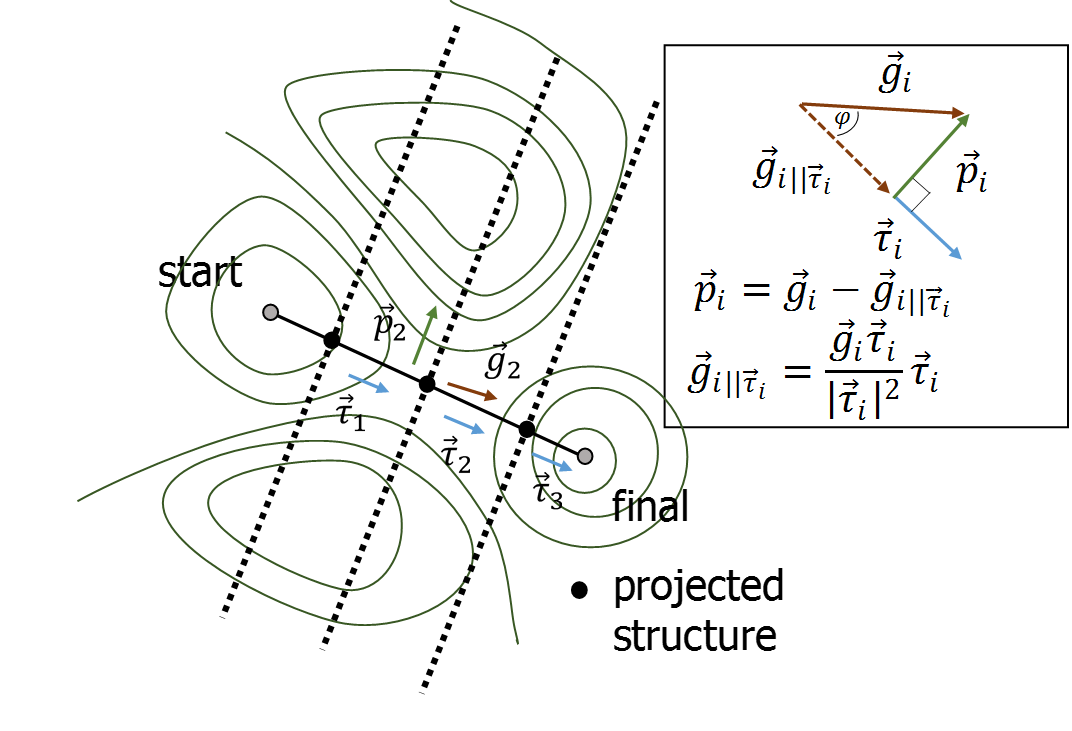
\includegraphics[scale=0.4]{img/MCM_scheme_new.png}\caption{Schematic representation of the Pathopt algorithm}
	\label{fig:MCM}
\end{figure}

\begin{figure}[h]
	\center
	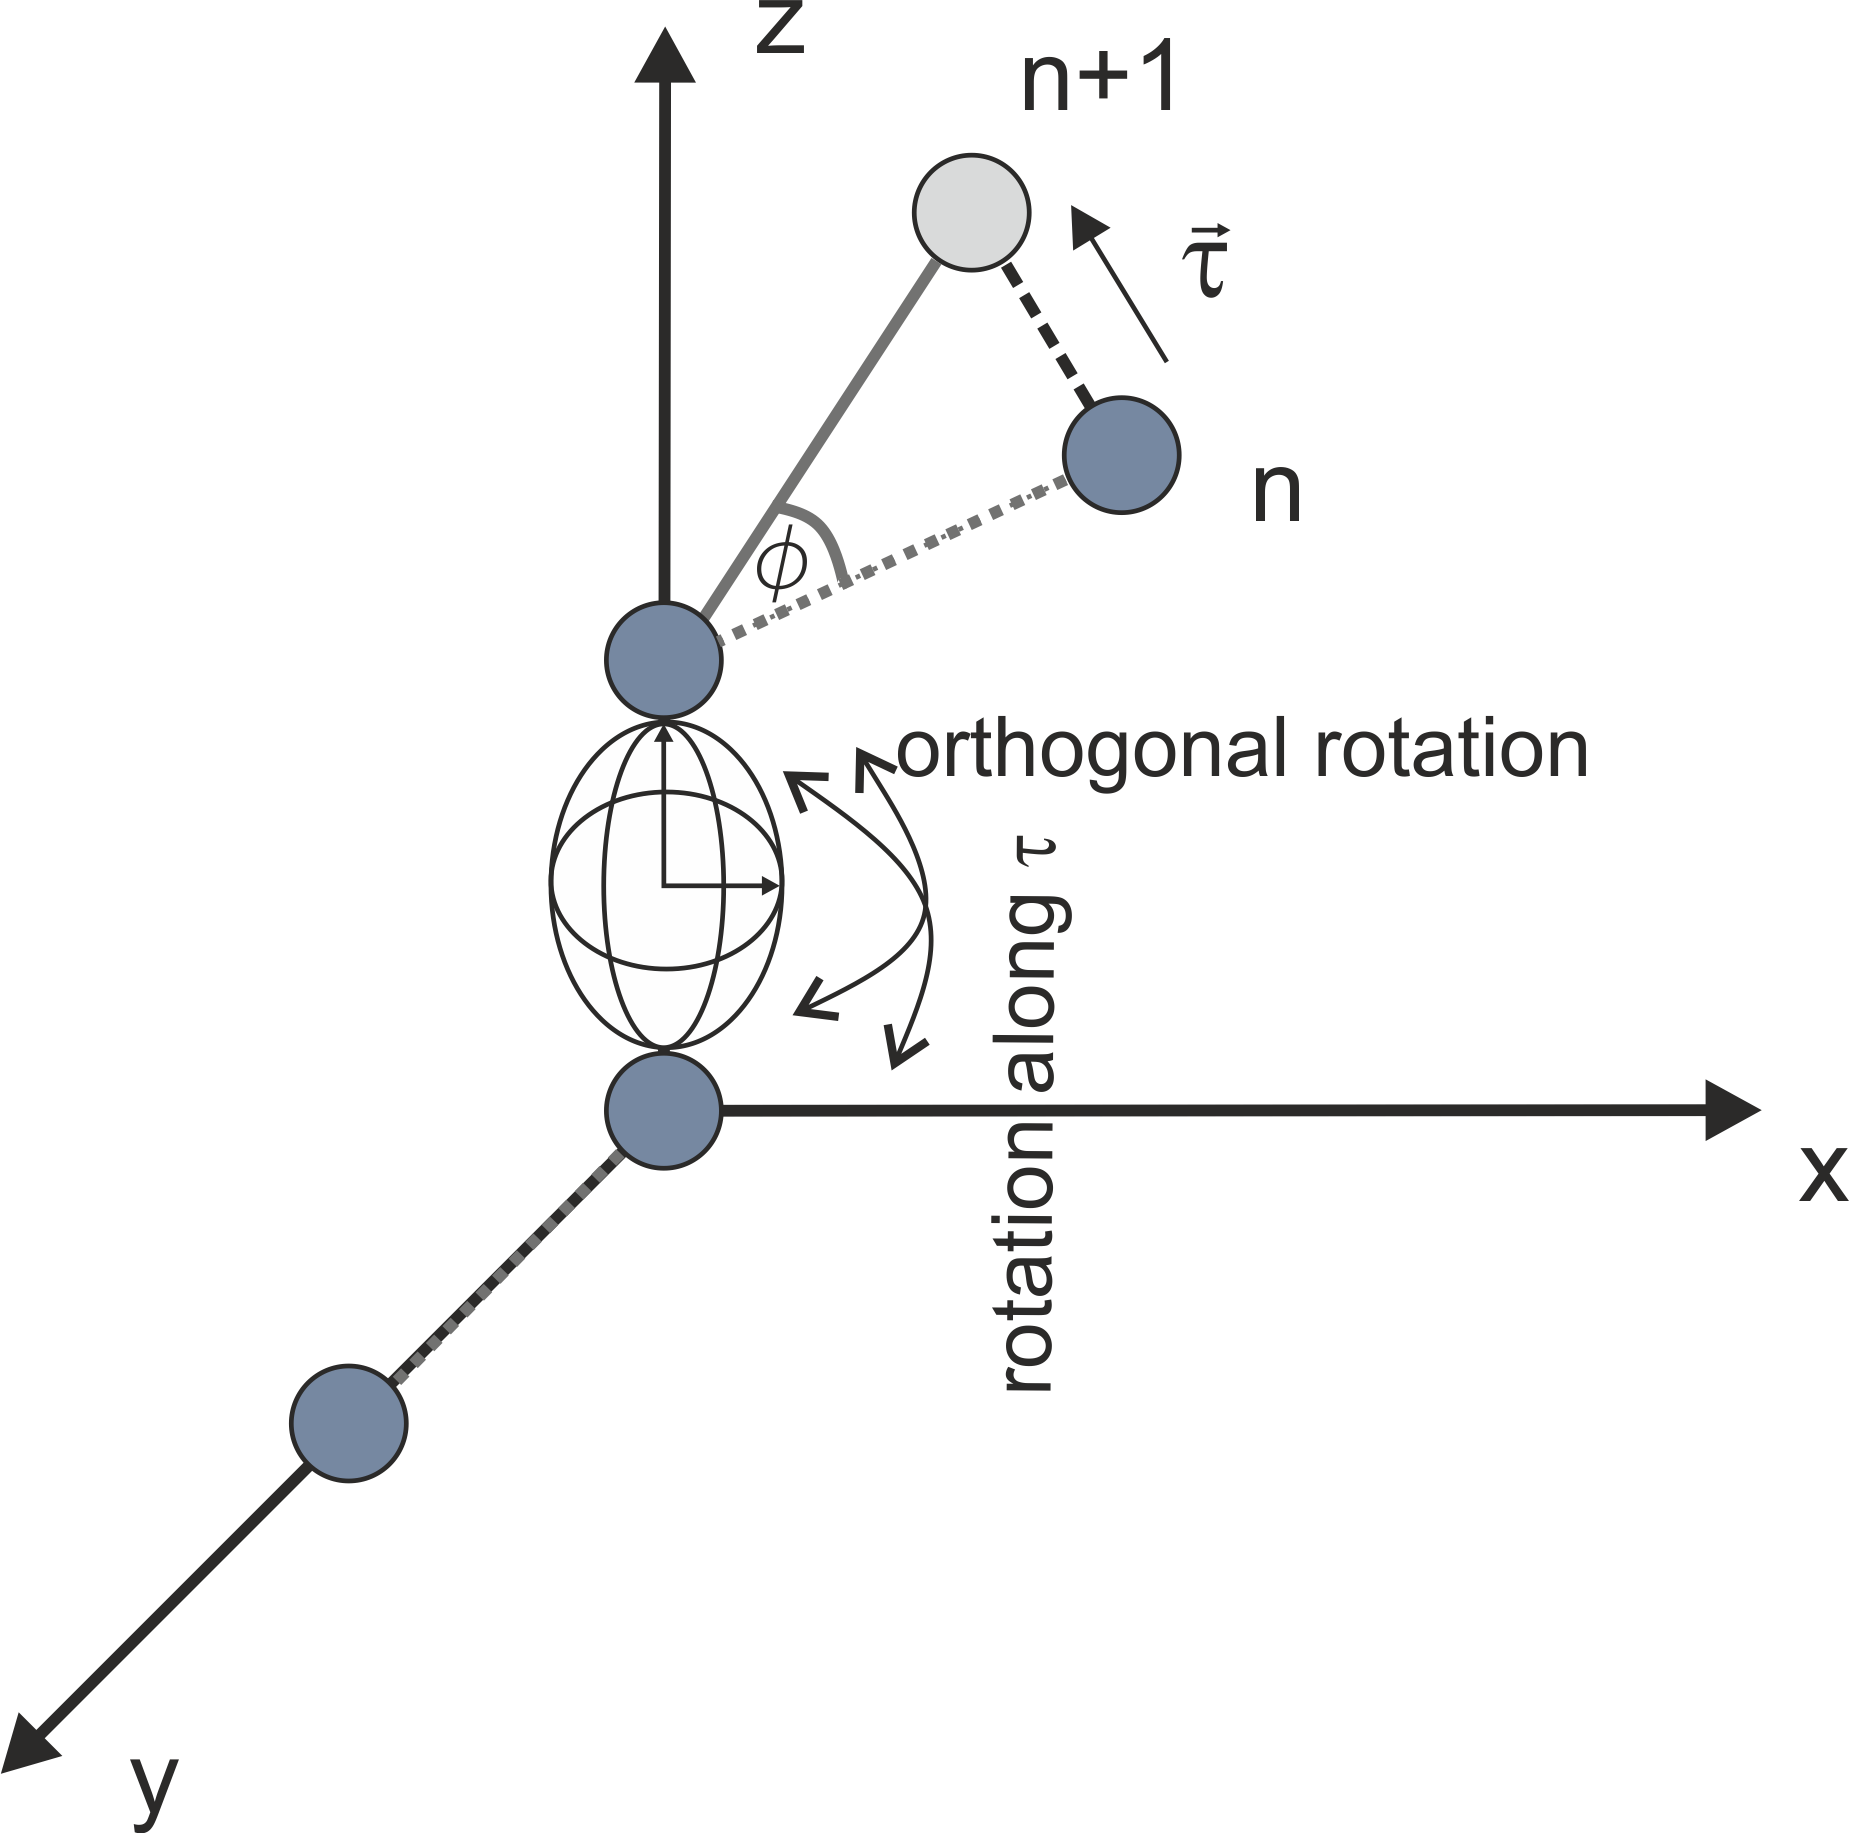
\includegraphics[scale=0.6]{img/grafik_rot_scheme.png}\caption{The mixed move strategy is illustrated by rotating only main dihedrals perpendicular to the connecting vectors $\tau$.}
	\label{fig:MIX}
\end{figure}

PO calculations can be carried out by using various optional configurations. For the MCM procedure within PO the following settings can be varied: Steps, number of total MCM runs, Temperature criterion, stepsize, acceptance criteria, move-type and optimization settings (standard L-BFGS settings are used e.g. convergence).
\begin{itemize}
	
	\item \texttt{NEB-PATHOPT-ITER} \textit{integer} - number of constraint MCM steps
	
	\item \texttt{NEB-PATHOPT-GLOBITER} \textit{integer} - number of total MC runs for multiple calculations
	
	\item \texttt{NEB-PATHOPT-TEMP} \textit{floating point value} - assigns temperature value in K
	
	\item \texttt{NEB-PATHOPT-STEPSIZE} \textit{floating point value} - Cartesian step size in $\AA$
	
	\item \texttt{NEB-PATHOPT-MAXVAR} \textit{floating point value} - maximum allowed displacement in $\AA$
	
	\item \texttt{NEB-PATHOPT-ENERGY\_RANGE} \textit{floating point value} - maximum allowed energy difference with respect to starting structure 
	
	\item \texttt{NEB-PATHOPT-MIXMOVE} \textit{bool} - de/-activates the dihedral movement approach
	
	\item \texttt{NEB-PATHOPT-MODE} \textit{character string} - assigns the gradient calculation scheme: PROJECTED=projected gradients / BIAS=bias potential
	
	\item \texttt{NEB-PATHOPT-BIAS} \textit{floating point value} - bias constant in kcal/mol$\AA^{2}$
	
	\item \texttt{NEB-PATHOPT-MF\_PATHOPT} \textit{bool} - de/-activates the temperature dependent MAXFLUX optimization of PO pathways (uses standard temp. criterion) 
	
\end{itemize}

After a successful PO calculation one should obtain the following files and folders: PATHOPT\_BASIN\_ENERGIES\_X.dat, PATHOPT\_STRUCTURES\_X\_Y.arc, arrhenius\_global.dat and folders 1-3. X and Y stand for the global run and concerning hyperplane.\newline

\begin{itemize}
	
	\item \texttt{PATHOPT\_BASIN\_ENERGIES} - contains the energies of the accepted structures with mcstep number, hyperplane number and energy in kcal/mol.
	
	\item \texttt{PATHOPT\_STRUCTURES} - contains the structures found on each hyperplane in TINKER format.
	
	\item \texttt{FOLDERS 1-3} - the connected pathways sorted as energy and structure files, whereas folder 1 contains next minimum RMSD moves along the hyperplanes and further on by increasing order.
	
	
	\item \texttt{arrhenius\_global.dat} - the arrhenius rates are given, but without any preexponential factor included.
	
\end{itemize}
	
	%%%% INTERNAL %%%%
	\subsection{INTERNAL - Conversion to internal coordinates}	
	The INTERNAL task converts cartesian coordinates to the internal coordinates used in CAST (z-matrix-like). The internal coordinates are then printed. This task can - for example - be run to identify dihedrals or angles which are to be constraint in a subsequent optimization task. \ac{PCA} task may be run on internal coordinates.

	%%%% STARTOPT %%%%
	\subsection{STARTOPT}	
	
	This task can be used to add water around a given molecule. To add a water box (for use of periodic boundaries) set the option SOtype to 1. The other possibility for this option is the Ringsearch\todo{what is RINGSEARCH doing?} task. Switch off periodic boundaries but set the boundary type SAboundary to 2 (box) and the SAradius to the desired boxsize. Pay attention that you give the correct atom types for the oxygen and hydrogen atoms in water (for the standard oplsaa forcefield those suggested in the inputfile are wrong) and decide if you want to optimize the water shell by the option SAopt. Then run the task STARTOPT.\\
	
	To use the outputstructure with periodic boundaries it is recommended to perform a LOCOPT run after adding the solvent box. So choose the task LOCOPT, switch on the periodic boundaries and set the box size in every direction to the size of your waterbox (SAradius) and run \ac{CAST} with the output of the START\-OPT task.\\
	
	Other options of this task are described in the following table:
	
	\begin{longtable}{|p{3.5cm}|p{5cm}|p{2.5cm}|}
		variable & effect & default \\
		\hline
    \textbf{\underline{Startopt Options}} &  &  \\ 
		\textbf{SOtype} & what kind of calculation will be performed? 
	\begin{itemize}
		\item 0 = Ringsearch
		\item 1 = Solvadd
		\item 3 = Ringsearch + Solvadd
	\end{itemize}	
	  & int [1]\\
		\textbf{SOstructures} & \todo[inline]{SOstructures} & ??? \\
		\hline
		\textbf{\underline{Solvadd Options}} & &  \\
		\textbf{SAhb} & \todo[inline]{SAhb} & float [1.8] \\
		\textbf{SAlimit} & number of water molecules that are added (0 = as many waters as needed for SAradius) & int [0] \\
		\textbf{SAboundary} & shape of the water shell \begin{itemize} \item 0 = layer\item 1 = sphere \item 2 = box \end{itemize} & integer [10] \\
		\textbf{SAradius} & size of the water shell (thickness of layer, radius of sphere or length of box) & float [10.0]\\
		\textbf{SAtypes} & force field parameter types of water oxygen and hydrogen & two integers \\
		\textbf{SAopt} & how is structure optimised? \begin{itemize} \item 0 = not at all \item 1 = after adding of each shell \item 2 = once after adding all waters \item 3 = each shell and all at the end \end{itemize} & int \\
		\textbf{SAfixinit} & fix initial structure during optimizations? (0 = no, 1 = yes) & int \\
		\hline
		\textbf{\underline{Ringsearch Options}} & \todo[inline]{Ringsearch options} &  \\ 
	\end{longtable}

	%%%% Free energy perturbation %%%%
	\subsection{FEP - Free Energy Perturbation}
	
\textbf{FEP only works with force field energy interfaces!!!}
	
	\acf{FEP} allows the alchemical transformation of one moiety into another and the derivation of the free energy change corresponding to the transformation. For \ac{FEP} calculations the coordinate file has to be slightly modified. \ac{CAST} uses the dual topology paradigm to define the topology for the chimeric system. In the dual topology paradigm both states of the transformation are present during the simulation. Therefore, the input structure of the starting system has to be extended by the moiety of the final structure. As an example, the transformation of ethane to propane is shown. \\

	\begin{figure}[h]
		\centering
		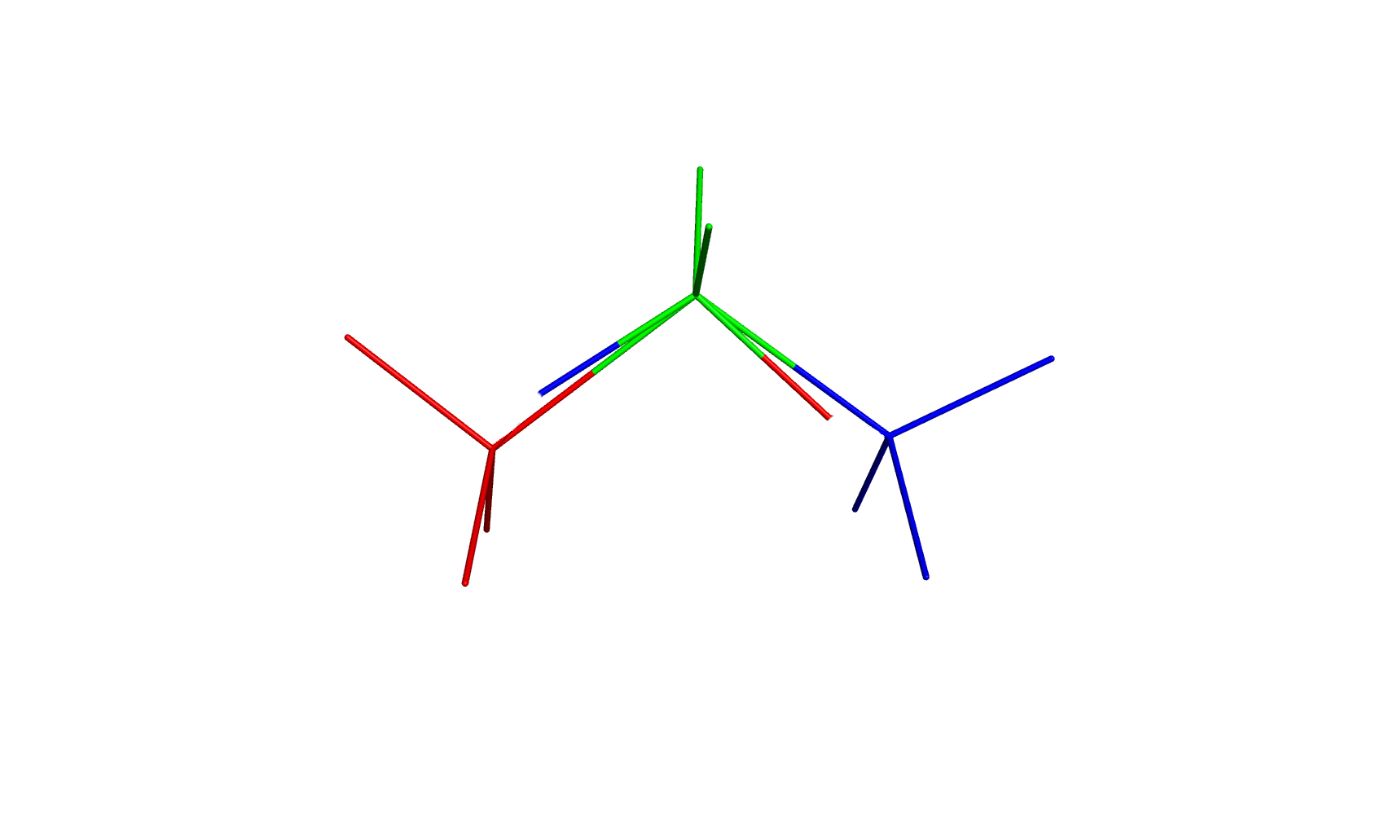
\includegraphics[width=0.5\textwidth]{img/imgfep1.png}
		\caption{Exemplifying \ac{FEP} calculations in \ac{CAST}}
		\label{fig:FEP1}
	\end{figure}
	The original ethane molecule inputfile is modified by adding another CH3-group + H to one of the ends of the molecule. In the next step the atoms belonging to both the starting and the final step have to be identified (they are marked in green in the figure). Those atoms don't need to be modified in the input file and are always present in the simulation. The atoms marked in blue are the ones belonging to the starting system and are phased ``out'' during the simulation. All atoms belonging only to the starting point have to be marked with an \textit{IN} in the coordinate file after the bonding partner specification. The atoms belonging to the final state of the system have to be marked with an \textit{OUT} after the bonding partner specification. The modified file is shown in the following:\\~\\
	\begin{figure}[h]
		\centering
		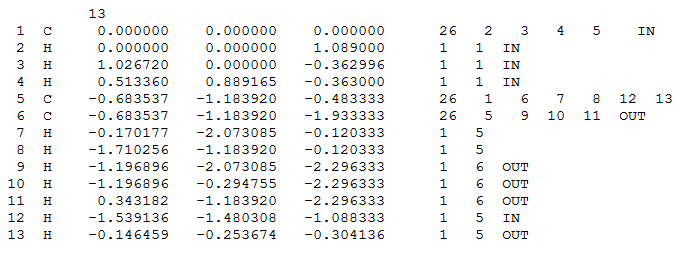
\includegraphics[width=0.95\textwidth]{img/imgfep2.png}
		\caption{Modifies tinker input style for \ac{FEP} calculations}
		\label{fig:FEP2}
	\end{figure}~\\
	One condition of the dual topology paradigm is that the atoms only belonging to the start point and end point must not interact with each other during the calculation. \ac{CAST} takes care of this automatically by excluding all angles, dihedrals or non-bonded interactions involving atom belonging to \textit{IN} or \textit{OUT}.\supercite{becker_development_2015}
	
	In order to avoid so called endpoint catastrophies the electrostatic and van der Waals-potentials between incoming and leaving atoms and static ones is modified \supercite{chipot_free_2007}
	
	The softcore electrostatic potential is:\supercite{becker_development_2015}
	\begin{align}
U_{el}(ab) = \lambda_{el} \cdot \frac{q_a \cdot q_b}{\sqrt[6]{R_{ab}^6 + \alpha_{cshift} \cdot (1-\lambda_{el})}} \label{cb_softcore}
\end{align}

The modified Lenard-Jones is calculated like this:\supercite{beutler_avoiding_1994}
\begin{align}
U_{vdw}(ab) = \lambda_{vdw} \cdot \epsilon_{AB} \left[ \frac{R_{ab,0}^{12}}{\left(\alpha_{vshift} \cdot (1-\lambda_{vdw})^2 \cdot R_{ab,0}^6 + R_{ab}^6 \right)^2}  -  \frac{2 \cdot R_{ab,0}^6}{\alpha_{vshift} \cdot (1-\lambda_{vdw})^2 \cdot R_{ab,0}^6 + R_{ab}^6}  \right] \label{LJ_softcore}
\end{align}
	
	
	\ac{FEP} calculations can be modified with various parameters:

	\begin{longtable}{|p{3cm}|p{5cm}|p{3cm}|}
		variable & effect & default \\
		\hline
		\textbf{FEPlambda} & Final value for order parameter. Doesn't need to be changed at all & float [1.0] \\
		\textbf{FEPdlambda} & Lambda increment. ${FEPdlambda}^{-1} =$ number of \ac{FEP} windows.	& float [0.05] \\
		\textbf{FEPvdwcouple} & Controls coupling of \ac{VdW} interactions $\lambda_{vdw,in} = \frac{\lambda}{FEPvdwcouple}$ for incoming atoms and $\lambda_{vdw,out} = \frac{1-\lambda}{FEPvdwcouple}$ for leaving atoms - both if the term is smaller than 1, else $\lambda_{vdw} = 1$ \supercite{_implementation_????} & float [1.0] \\
		\textbf{FEPeleccouple} & Controls coupling of electrostatics \mbox{$\lambda_{el, out} = 1- \frac{\lambda}{1-FEPeleccouple}$} for leaving atoms and \mbox{$\lambda_{el, in} = 1- \frac{1-\lambda}{1-FEPeleccouple}$} for incoming atoms - both if the term is bigger than 0, else $\lambda_{el} = 0$ \supercite{_implementation_????}
		& float [1.0] \\
		\textbf{FEPvshift} & Value for the \ac{VdW} shifting parameter in the softcore potential ($= \alpha_{vshift}$ in equation \ref{LJ_softcore}) & float [1.0] \\
		\textbf{FEPcshift} & Value for shifting parameter in the electrostatic potential ($= \alpha_{cshift}$ in equation \ref{cb_softcore}) & float [1.0] \\
		\textbf{FEPequil} & Number of equilibration steps in each window & integer [10] \\
		\textbf{FEPsteps} & Number of production steps in each window & integer [10]\\
		\textbf{FEPfreq} & Frequency of \ac{FEP} output & integer [1] \\
		\textbf{FEPanalyze} & switch on or off analyzing of FEP calculation (0 or 1) & bool [1] \\
		\textbf{FEPbar} & switch on or off calculating $\Delta G$ from Bennets Acceptance Ratio (BAR) (0 or 1)  & bool [0] \\
	\end{longtable}

	\ac{FEP} calculations produce two output files: ``alchemical.txt'' and ``FEP\_Results.txt''. ``alchemical.txt'' contains detailed information about electrostatic and \ac{VdW} interactions for the current lambda value. Furthermore, the temperature and free energy change is displayed. The columns are:
	\begin{itemize}
	\item electrostatic interactions for $\lambda - \Delta \lambda$
	\item electrostatic interactions for $\lambda$
	\item electrostatic interactions for $\lambda + \Delta \lambda$ (in the file also called dLambda)
	\item Van der Waals interactions for $\lambda - \Delta \lambda$
	\item Van der Waals interactions for $\lambda$
	\item Van der Waals interactions for $\lambda + \Delta \lambda$ 
	\item temperature
	\item $\Delta E_{pot} = U(\lambda + \Delta \lambda) - U(\lambda)$
	\item $\Delta G$ calculated from a forward transformation out of $\Delta E_{pot}$
	\item $\Delta E_{pot, back} = U(\lambda) - U(\lambda - \Delta \lambda)$
	\item $\Delta G_{back}$ calculated from a backward transformation out of $\Delta E_{pot,back}$
	\end{itemize}
	The free energy changes in the lines without columns are only from the forward transformation.
	
	The file ``FEP\_Results.txt'' contains the total free energy change for the simulation and for each window. The first column is the $\lambda$-Value where the current window ends, the second line the total free energy change until this window from the forward transformation, the third line the total free energy change until this window from the backward transformation. The total free energy changes for forward and backward simulation should be similar (in theory identical). The fourth line is the total free energy from Simple Overlap Sampling (SOS), a combination of forward and backwards transformation. If you have switched on BAR the results for the BAR calculation are in the fifth column. Otherwise this column is filled with zeros.
	
	If you have switched on FEPanalyze for every window the probability distributions of $\Delta E_{pot}$ are plotted for the forward and backwards transformation and saved as a .png image. Furthermore the overlap of these distributions is calculated and written into a file ``overlap.txt''. The quality of a calculation is better if the overlap is bigger, i.\,e. the distributions for forward and backwards transformation are similar. To perform such an analysis CAST has to be compiled with python. See section \ref{sec:compile} for a description how to do this. Python needs the module ``matplotlib''. Furthermore the file ``FEP\_analysis.py'' has to be provided (compare section \ref{sec:DFTB}). 
	
	The \ac{FEP} implementation is part of the \ac{MD} code. Thermostats, barostats boundary conditions and all other parameters needed can be controlled with the corresponding \ac{MD} variables.
	
	If you use a temperature gradient it will only be applied in the initialisation run but not in the equilibration and production runs. In those the temperature is kept constant at the last temperature of your gradient.
	
\textbf{Attention!} The fact that during an FEP run several MD simulations with possibly different settings are done can cause some problems you should be aware of: \\
For example if your ``MDsteps'' is 1000, ``FEPequil'' is 10000 and ``FEPsteps'' is 50000 you will have MD runs with 1000 (for the initialisation at the very beginning), 10000 (for the equilibration of every FEP window) and 50000 steps. The stepsize between two snapshots is however calculated from the number ``MDsteps''. So if in the above example ``MDsnap'' is 1000 the program will will calculate the stepsize so that a snapshot is taken for every MD step not only in the initialisation MD with 1000 steps but also in every equilibration run with 10000 steps and in every production run with 50000 steps. So it is strongly recommended to set the ``MDsnap'' option to a very low number when doing an FEP calculation in order to avoid getting snapshot files that are much too big to deal with. \\

	
	%%%% Trajectory alignment (ALIGN) %%%%
	\subsection{ALIGN - Trajectory Alignment}
	\label{sec:align}
	The trajectory alignment task allows the alignment of ensembles of structures, for example structures obtained from molecular dynamics. For translational alignment, the center-of-mass of all structures are aligned to the origin of the coordinate system. Rotational alignment is performed via Kabsch's method\supercite{kabsch1, kabsch2}. This task can furthermore calculate distance measures between the structures of the ensemble in regard to a reference structure. Regarding the distance metric, one can chose between the (standard) \ac{RMSD}, the \ac{dRMSD} and the Holm and Sander Score\supercite{holmsander}. For a comparison of molecular distance meassures see \cite{distancemeasures}. If no alignment is performed beforehand the distance measures are calculated among the unaligned snapshots. \ac{CAST} provides the following options for the task ALIGN: \\~\\
	
	\begin{longtable}{|p{3.5cm}|p{5cm}|p{2.5cm}|}
		variable & effect & default\\
		\hline
		traj\_align\_translational & Switch translational (= center-of-mass) alignment on or off, false = off, true = on & true\\
		traj\_align\_rotational & Switch rotational alignment\cite{kabsch1, kabsch2} on or off, false = off, true = on & true\\
		traj\_print\_bool & Switch output of distance measurement on or off, ``false'' = off, ``true'' = on & true\\
		align\_external\_file & Get reference structure from different file then to-be-aligned structures. This is the filename. The file has to be in the same folder. & none\\
		ref\_frame\_num & Number of reference frame for alignment (if align\_external\_file is used, this number refers to the therby specified ensemble). First structure is ``0'' & 0\\
		dist\_unit & Specifies the distance metric; 0 = RMSD, 1 = dRMSD, 2 = Holm and Sander Score & 0\\
		holm\_sand\_r0 & value for Holm and Sander Score's contact cutoff distance in \AA & 20 \\
		
	\end{longtable}
	
	%%%% Entropy calculations (ENTROPY) %%%%
	\subsection{ENTROPY - Conformational and Configurational entropy calculations}
	For further analysis of \acl{MD} ensembles \ac{CAST} provides the calculation of entropy contributions. Different approaches for entropy calculation can be used. Currently \ac{CAST} offers calculations according to Karplus\supercite{karplus_entropy}and Schlitter\supercite{schlitter_entropy}. Entropy calculations according to Karplus are modified from the original publication, as some minor math errors have been fixed. Calculations can be performed in cartesian or internal coordinates for all or only several snapshots. Furthermore, the \acp{DOF} can also be truncated to a selection of internals or cartesian coordinates. If internal coordinates are to be used, you need to specify the indentifying integer of the atom where the desired internal coordinate belongs to. Since the building of internal Z-Matrices can differ between different software packages, we suggest you run the task ``INTERNAL'' to obtain the Z-Matrix \ac{CAST} will use for your specific molecular system. The following options are provided by \ac{CAST}: \\~\\
	
	\begin{longtable}{|p{4cm}|p{5cm}|p{2cm}|}
		variable & effect & default\\
		\hline
		entropy\_alignment & Switch alignment of structures according to Kabsch's method\cite{kabsch1, kabsch2} on or off, false = off, true = on; see section \ref{sec:align} & true\\
		entropy\_ref\_frame\_num & Reference frame for alignment & 0 \\
		entropy\_start\_frame\_num & First frame to be used for entropy calculations & 0 \\
		entropy\_offset & If a value \textit{n} $\neq 1$ is specified, only every \textit{n'th} frame will be used for entropy calculations & 1 \\
		entropy\_temp & Temperature of the original simulation in K & 300.00 \\
		entropy\_use\_internal & Specifies wether internal coordinates should be used, ``true'' = yes, ``false'' = ``no'' & false \\
		pca\_use\_internal & Specifies wether internal coordinates should be used, ``true'' = yes, ``false'' = no & false \\
		entropy\_internal\_ang & Specify number of atoms (starting with ``0'') for which the bond angle in radians will be included in the entropy calculations (example: ``3-7,8,13,15,79-115'') & none\\
		entropy\_internal\_bnd & Specify number of atoms (starting with ``0'') for which the dihedral angle will be included in the entropy calculations (example: ``3-7,8,13,15,79-115'') & none\\
		entropy\_trunc\_atoms\_bool & If cartesian coordinates are used, this specifies wether only those belonging to certain atoms will be used in entropy calculations. Options are ``true'' = truncation activated and ``false'' = all atoms will be included. & false\\
		entropy\_trunc\_atoms\_num & If entropy\_trunc\_atoms\_bool = true, specify the integers of those atoms whose coordiantes are to be included (example: ``1,3,7,11-45,2,77-99'') & none\\
		entropy\_method & Specifies the method according to which the entropy will be calculated 
		\begin{itemize}
		\item 1 = Quasi-Harmonic-Approx., configurational entropy, according to Karplus\supercite{karplus_entropy}
		\item 6 = Quasi-Harmonic-Approx., conformational entropy, according to Schlitter\supercite{schlitter_entropy} (use with cartesian coordiantes only)
		\item 0 = All of the above, executed sequentially
		\end{itemize}\\
		
	\end{longtable}
		
	%%%% Principal Component Analysis (PCA) %%%%
	\subsection{PCA - Principal Component Analysis}
	The \acl{PCA} tasks performs a principal component analysis on Simulation trajectories. The procedure is split into two tasks, \textit{PCAgen} and \textit{PCAproc}. First, \textit{PCAgen} is run to obtain the coordinates of the input trajectory in their transformed form as \ac{PCA} modes. These are contained in a file titled ``pca\_modes.dat'' which also contains the eigenvalues and eigenvectors of the covariance matrix. For more information on the theoretical background of the use of \ac{PCA} see \cite{pca_review, pca_review2, dpca1, dpca2, dpca3}. The mathematical steps in performing \ac{PCA} are closely related to those during conformational and configurational entropy calculations, therefore the configuration options of this task are very similar to those of the task ENTROPY:
	
	\begin{longtable}{|p{3.5cm}|p{5cm}|p{2.5cm}|}
		variable & effect & default\\
		\hline
		pca\_alignment & Switch alignment of structures according to Kabsch's method\cite{kabsch1, kabsch2} on or off, false = off, true = on; see section \ref{sec:align} & true\\
		pca\_ref\_frame\_num & Reference frame for alignment & 0 \\
		pca\_start\_frame\_num & First frame to be used (couting starts at ``0'') & 0 \\
		pca\_offset & If a value \textit{n} $\neq 1$ is specified, only every \textit{n'th} frame will be used & 1 \\
		pca\_read\_vectors & Switch ``true'' or ``false''. If ``true'', eigenvectors of the covariance matrix will not be calculated but read from a previously performed \ac{PCA} file named \glqq pca\_modes.dat\grqq. This enables the projection of structures onto the \ac{PCA} modes of other trajectories. & "false" \\
		pca\_read\_modes & Switch ``true'' or ``false''. If ``true'', \ac{PCA} Modes of the covariance matrix will not be calculated but read from a previously performed \ac{PCA} file named \glqq pca\_modes.dat\grqq. This is for example useful when different histogramming procedures are to be applied. & ``false'' \\
		pca\_use\_internal & Should dihedrals instead of cartesian coordinates be used? & ``false''\\
		pca\_internal\_dih & Specify number of atoms (starting with ``1'') for which the dihedral angle in radians will be included in the dPCA according to task INTERNAL (see \cite{dpca1, dpca2, dpca3}) (example: ``3-7,8,13,15,79-115'') & none\\
		pca\_ignore\_hydrogen & Ignore either all cartesian coordinates of hydrogens or all dihedrals including hydrogen & ``false'' \\
		pca\_trunc\_atoms\_bool & If cartesian coordinates are used, this specifies weather only those belonging to certain atoms will be used in the\ac{PCA}. Options are ``true'' = truncation activated and ``false'' = all atoms will be included. & false\\
		pca\_trunc\_atoms\_num & If pca\_trunc\_atoms\_bool = true, specify the integers of those atoms whose coordinates are to be included (example: ``1,3,7,11-45,2,77-99'') & none\\
		\end{longtable}
		~\\
		\begin{longtable}{|p{5.1cm}|p{5cm}|p{1cm}|}
		variable & effect & default\\
		\hline
		pca\_print\_probability\_density & Boolean flag (``true'' / ``false'' ): Print probability density of generated PCA modes (obtained through internal histogramming). & true\\
		pca\_histogram\_width & Bin size of one histogram. Number of bins is adjusted accordingly. One can use ``pca\_histogram\_number\_of\_bins\ alternatively. & none\\
		pca\_histogram\_number\_of\_bins & Number of histogram bins per dimension. Bin size is adjusted accordingly. ``pca\_histogram\_width'' can be used alternatively. & none\\
		pca\_dimensions\_for\_histogramming & Specify an integer range identifying the dimensions that will be histogrammed. Alternativly, write "all" to obtain one-dimensional hisograms of all dimensions. Example: ``1,2'': Two dimensional histogramming of the first two \ac{PCA} Modes. Example: ``1-3'': Three-Dimensional histogramming of the first three \ac{PCA} Modes. Example: ``1,5,8,11-15'' etc.& none\\
		
	\end{longtable}~\\
		
	 \ac{CAST} will, after performing \ac{PCA}, perform histogramming of \ac{PCA} modes as desired by the user to get an approximation to the free energy landscape of the molecular system. Usually, one would want to histogram the first two \ac{PCA} modes to obtain a two-dimensional approximation to the free energy landscape. An example for the configuration flags for the most common application of (cartesian) \ac{PCA} through \ac{CAST} is:\\
	 
	 \begin{lstlisting}
	 pca\_alignment                     true
	 pca\_ref\_frame\_num                 0
	 pca\_start\_frame\_num               0
	 pca\_read\_vectors                  false
	 pca\_read\_modes                    false
	 pca\_print\_probability\_density     true
	 pca\_histogram\_width               0
	 pca\_histogram\_number\_of\_bins      100
	 pca\_dimensions\_for\_histogramming  1,2\end{lstlisting}
	 
	 The output of the histogramming is placed in a file called ``pca\_histograms''. For the above example of two-dimensional histogramming, the output can be easily plotted using gnuplot\cite{gnuplot_4.4}. Example options for gnuplot are given below:\\
	 \begin{lstlisting}
	set terminal png
	set output ``pca_hist.png''
	set pm3d map
	splot ``pca\_histograms.dat''\end{lstlisting}~\\	
	
	From this plot, one can identify basins of the \acl{PES}. To obtain the structures corresponding to those basins, the second task \textit{PCAproc} may be used. It reads the file \textit{pca\_modes.dat} and the original input ensemble to extract structures corresponding to desired regions of the histogrammed \ac{PCA} Modes. It is important to note that in this task coordinates are regained from the PCA-modes via an unitary transformation. Then, they are matched to the full input-trajectory. Therefore, options such as \textit{pca\_start\_frame\_num} or \textit{pca\_offset} are ignored for the \textit{PCAproc} task. Input options for this task are the following:\\~\\~\\
	\begin{longtable}{|p{3.5cm}|p{5cm}|p{2.5cm}|}
		variable & effect & default\\
		\hline			
		proc\_desired\_start & Float values, each one corresponding to the start of a desired region in one dimension (Example:'' -5.0, -1.0'') & none\\
		proc\_desired\_stop & Float values, each one corresponding to the stop of a desired region in one dimension (Example:'' 5.0, 6.0'') & none\\
	\end{longtable}

	%%%%INTERFACE_CREATION%%%%
	\subsection{INTERFACE CREATION}
	The INTERFACE\_CREATION task uses as input besides the standard structure information an additional input for a second structure denoted by the keyword \textit{ICname}. Furthermore the type of the input file is necessary. Like for the standard input, only tinker and amber are implemented as file types. The choice has to be put at the \textit{ICinputtype} option. Furthermore the task requires an input of the dimension along which the structures shall be put together, only \textit{x}, \textit{y} or \textit{z} are possible, and the distance between the structures. These options are determined by the keywords \textit{ICaxis} and \textit{ICdistance}, respectively. The used unit for the distance is \aa ngström.\\
With the input depicted below the structures are combined to yield a new system .

\begin{lstlisting}
#Creation of a new Structure from the usual input 
#structure and an additional one

#Additional input file name

ICname             fultri.xyz

#Additional input file type 

ICinputtype         TINKER

#From which axis should the additional atoms added 

ICaxis              y

#How far apart should they be 

ICdistance           4.0
\end{lstlisting}


	%%%%CENTER%%%%
	\subsection{CENTER}
	
	The options for the CENTER task are limited since the names for the output files are hard coded to ensure smoother usage of the files in the following COUPLINGS task. With the first option denoted by the keyword \textit{CENTERdimer} the user decides if, additionally to the centers of mass, dimer structure pairs should be generated.
For this option a \textit{0} means only the centers of mass are to be calculated and a \textit{1} means the dimer pairs are also to be created. The \textit{CENTERdistance} keyword is only used when dimer structures are generated. With it the user defines the maximum distance between the centers of mass for which a dimer structure is generated. The distance has to be given in \aa ngström.\\
\begin{lstlisting}
#Calculation the centers of mass for all molecules
#in the System options only used to determine dimer criteria

CENTERdimer                     1


CENTERdistance                  15.0 
\end{lstlisting}

	%%%%COUPLINGS%%%%
	\subsection{COUPLINGS}
	
	The dimer pairs created by the previously discussed task can be put to use in the COUPLINGS task and are perfectly suited for it, as they are already named in the fashion required by the COUPLINGS task. The required numbers of p-type and n-type semiconductor monomers are to be put in at the \textit{CouplingspSCnumber} and \textit{CouplingsnSCnumber} keywords, respectively.\\
The option \textit{CouplingsCTcharastates} is used to define the excited states to be considered for the charge transfer process at the interface and thus the calculation of the charge transfer coupling.\\
The remaining options specify the Gaussian09\supercite{M.J.Frisch2009} options to be used for the correspondent calculation. The keywords \textit{CouplingspSCdimMultiplicity}, \textit{CouplingsnSCdimMultiplicity} and \textit{CouplingsheterodimMultiplicity} are for the specification of the multiplicity the different dimer types possess. The options \textit{CouplingspSCdimCharge}, \textit{CouplingsnSCdimCharge} and \textit{CouplingsheterodimCharge} do the same for the charges of the dimer structures.
The methods to be used for the couplings calculations are specified with the keywords \textit{CouplingspSCdimElCalcmethod} for the electron transport coupling, \textit{CouplingspSCdimExciCalcmethod} for the exciton transport coupling, \textit{CouplingsnSCdimholCalcmethod} for the hole transport coupling and \textit{CouplingsheterodimCalcmethod} for the charge transport couplings, electron transfer and recombination. It must be noted that the options for \textit{CouplingspSCdimExciCalcmethod} and \textit{CouplingsheterodimCalcmethod} must specify an excited states calculation. The other methods must be ground state calculations.\\

\begin{lstlisting}
#Calaulation of couplings  needed for XB_EXCITONBREAKUP

#Number of p-type semiconductor monomers

CouplingspSCnumber                    6

#Number of n-type semiconductor monomers        

CouplingsnSCnumber                    3 

#List of states relevant for ct-processes (no comma)

CouplingsCTcharastates                3 4 7

#p-type homodimer options

CouplingspSCdimMultiplicity           1  

CouplingspSCdimCharge                 0  

CouplingspSCdimElCalcmethod           INDO 

CouplingspSCdimExciCalcmethod         ZINDO TD=(NStates=9,Singlets,  													 		   AllTransitiondensities,															 					ListWindow) gfinput 																					IOP(6/7=3) 

#n-type homodimer options

CouplingsnSCdimMultiplicity           1 

CouplingsnSCdimCharge                 0 

CouplingsnSCdimholCalcmethod          INDO 

#heterodimer options

CouplingsheterodimMultiplicity        1 

CouplingsheterodimCharge              0 

CouplingsheterodimCalcmethod          ZINDO TD=(NStates=9,Singlets, 																 AllTransitiondensities, 																			  ListWindow)gfinput 																					  IOP(6/7=3) 
\end{lstlisting}
In the exemplary input the methods for the excited states calculations are written in more than one line, this is not the case in the used input file, but was necessary in this work to ensure legibility. \\
The Gaussian keywords used for the calculations employed in this work are explained here as some of them are not encountered very often. With the command \textit{TD} an calculation for the excited states is requested in Gaussian, the option \textit{NStates} is used to declare the number of excited states calculate and the keyword \textit{Singlets} ensures only singlet excited states are considered. The method for the calculation of the charge transfer and recombination couplings in the heterodimer must furthermore include the \textit{AllTransitiondensities} keyword for Gaussian, so that the electric transition dipole moments between all states, not only the moments concerning the ground state, are written in the Gaussian output file so CAST can read them. Another not broadly used Gaussian commands is the \textit{IOP(6/7=3)} keyword, which here reads, set option 7 in overlay 6 to 3, which makes Gaussian write out all MO's. The keyword \textit{gfinput} tells Gaussian to print the used basis set in a way so it can be used as a general basis set. A list of orbitals from the input can be frozen by usage of the \textit{ListWindow} keyword in Gaussian.\\
The calculated couplings are written once in a file called ``Couplings.txt'' in the order couplings of the p-type semiconductor homodimers, then the couplings of the heterodimers and finally the couplings of the n-type semiconductor pairs. Additionally, the couplings of the three kinds of dimers are also written into three separate files called ``homodimer\_exciton.txt'', ``homodimer\_ladung.txt'', ``heterodimer.txt'' and ``nSC\_homodimer.txt'' with names corresponding to the contained information. \\
In the files, first the indices of the monomers are written, then the associated couplings. In the ``Couplings.txt'' for the p-type semiconductor dimers the couplings in the third column are the electron transport coupling whereas the exciton transport couplings are in the fourth column. Furthermore, are the charge transfer couplings in the third column and the recombination couplings in the fourth column for the heterodimers in both the ``Couplings.txt'' and ``heterodimer.txt''.

	%%%%EXCITON_BREAKUP%%%%
	\subsection{EXCITONBREAKUP}
With the keyword \textit{EXmasscenters} the name of the file containing the centers of mass is denoted, the numbers of p- and n-type semiconductors are to be given at the \textit{EXnumberp} and \textit{EXnumbern} options, respectively. At the \textit{EXplaneinterf} keyword the dimension ($x, y$ or $z$) perpendicular to the interface plane has to be specified. \\
The files containing the couplings must be given at the keywords \textit{EXpscpairexrates} for the exciton transport couplings, \textit{EXpscpairchrates} for the electron transport couplings, \textit{EXpnscpairrates}, for the couplings of the heterodimers and \textit{EXnscpairrates} for the hole transport couplings.\\
The input for the recombination energies involved in the various processes are denoted with the keywords \textit{EXReorgE\_exc} for the exciton transport, \textit{EXReorgE\_ch} for the electron transport, \textit{EXReorgE\_nSC} for the hole transport, \textit{EXReorgE\_ct} for the charge transfer and \textit{EXReorgE\_rek} for the reorganisation. The keywords are chosen in a fashion so they reflect which reorganisation energy is needed there. The driving forces for charge transfer and recombination are necessary at the keywords \textit{EXct\_triebkraft} and \textit{EXrek\_triebkraft}, respectively. The recombination energies and driving forces all are in the unit electronvolt. The parameters necessary to calculate the fluorescence rate are requested at the keywords \textit{EXoscillatorstrength}, for the oscillator strength, and \textit{EXwellenzahl}, for the wavenumber. The wavenumber is used in the unit inverese centimeter.
\begin{lstlisting}
#Input for simultion of exciton behaviour at 
#an semiconductor interface.

#Center of masses of all semiconductor molecules

EXmasscenters                 CenterofMasses.out

#Numbers of monomers

EXnumbern                     3

EXnumberp                     6

#Orientation of the interface

EXplaneinterf                 y

#Couplings for all possible dimers

EXnscpairrates                nSC\_homodimer.txt

EXpscpairexrates              homodimer\_exciton.txt

EXpscpairchrates              homodimer\_ladung.txt

EXpnscpairrates               heterodimer.txt

EXReorgE\_exc                 0.561

EXReorgE\_ch                  0.194

EXReorgE\_nSC                 0.178

EXReorgE\_ct                  0.156

EXReorgE\_rek                 0.184

EXct\_triebkraft              1.550

EXrek\_triebkraft            -4.913

EXoscillatorstrength          0.0852

EXwellenzahl                  28514.91
\end{lstlisting}	
	
	%%%% GRID %%%%
	\subsection{GRID - ?}	
	\todo[inline]{write something about task GRID}
	
	%%%% PATHSAMPLING %%%%
	\subsection{PATHSAMPLING - ?}	
	\todo[inline]{write something about task PATHSAMPLING} 	
	
	\subsection{SCAN2D - ?}	
	\todo[inline]{write something about task SCAN2D} 	
	
	%%%% REMOVE_EXPLICIT_WATER %%%%
	\subsection{REMOVE\_EXPLICIT\_WATER}	
	This task will remove all explicit water from the input trajectory and write out the truncated coordinate. This may be useful to prepare data for tasks such as ENTROPY, PCAgen or ALIGN. In detail, the truncation is performed by detecting oxygen atoms which are only bound to two hydrogen atoms.\\
	
	\subsection{WRITE\_TINKER}
	This task writes out the tinkerstructure into the file \textit{outname}.arc. If your inputfile is also a tinkerstructure this task is not of much use because input and output are identical (but the output is perhaps formated more nicely). But if your inputfile is of another type, e.\,g. XYZ you can convert it to a tinkerfile (see also section \ref{sec:tinker}).
	
	\subsection{WRITE\_XYZ}
	This task writes the inputstructure into a xyz-file \textit{outname}.xyz. It can be used to convert coordinates from another inputformat or just to get a nicer formatting of an already existing xyz-file.
	
	\subsection{WRITE\_GAUSSVIEW}
	This task writes a file that you can open with gaussview. It is meant to help you with finding the correct atom numbers for your QM- and SE- atoms in a QM/MM or three-layer calculation or get a better view at existent layers.
	\textbf{WARNING!} Though the file that is created is technically a gaussian inputfile it is not meant to be used to run gaussian calculations because a lot of input is filled by random stuff. CAST only takes the atom information (element and coordinates) and -- if QMMM, ONIOM or THREE\_LAYER is given as energy interface -- the information which atom belongs to which layer.
	
	You can open the resulting .gjf file with gaussview. To show the atomic numbers by clicking View $\rightarrow$ Labels. To play around with QM/MM layers open Tools $\rightarrow$ Atom Groups. Then under "`Atom Group Class"' select "`ONIOM Layer"'.
	
	\subsection{WRITE\_PDB}
    This task writes a .pdb file of an inputstructure which you can open in pymol. This is especially useful for protein structures as you can display the aminoacid sequence in pymol and look at the aminoacids that are particularly interesting to you. 
    \textbf{WARNING!} Not all fields in the pdb file are filled so not all functionality of pymol might work on the created structures!
	
	\subsection{MODIFY\_SK\_FILES}
	This task converts DFTB parameter files from the dftb.org format to the format needed by gaussian16. For details of the conversion see \cite{noauthor_dftbgaussian_nodate}, Modifying Slater-Koster Files. In order to perform a DFTB calculation gaussian needs parameters for every pair of elements in the input structure. So for every pair of elements in your input structure you need to provide CAST with a parameter file. Those files can be downloaded here: \url{http://www.dftb.org/parameters/download/}. CAST takes the structure, looks which element pairs are present and converts the files. If there is an element pair in your structure for which no parameter file is provided CAST gives a warning. The old parameter files are deleted and replaced by the new ones. These can be used for gaussian calculations.
	
\textbf{Important!} If you run this task the symbol column of the tinkerfile has to contain the element symbol and nothing else. Otherwise CAST is not able to find the correct element pairs!

\subsection{MOVE\_TO\_ORIGIN}

This task moves your structure to the origin of the coordinate system. Either the center of mass or the center of geometry are moved to the origin, i.\,e. the point (0/0/0) in the cartesian coordinate system. Which of those two options happens can be determined by the user with the option \texttt{MOVEmode} in the inputfile \texttt{CAST.txt}.
		

	%%%% Boundry Conditions %%%%
	\section{Boundary Conditions}
	\label{sec:boundary}
	\ac{CAST} features two types of boundary conditions: spherical and periodic. Spherical boundary conditions can be applied with an energy interface if desired, periodic boundaries are limited to the force field interfaces.

	%% Spherical boundaries
	\subsection{Spherical boundaries}
	Spherical boundaries apply a harmonic potential on particles which drift farer away from the geometric center of the simulation than a certain threshold. There are 7 input parameters in total which are defined in a single line in the input file. \\~\\

	\begin{longtable}{l|l|l|l|l|l|l|l}
		keyword & param1 & param3 & param4 & param5 & param6 & param7 \\
		\hline
		MDspherical & active & Radius1 & Radius1 & Force1 & Force2 & Exp1 & Exp2 \\
		MDspherical & 1 & 30.0 & 0.0 & 10.0 & 0.0 & 2 & 0 \\
	\end{longtable}~\\

	Effects of the input variables in detail:
	\begin{longtable}{|p{3cm}|p{5cm}|p{3cm}|}
		\textbf{variable} & effect & default \\
		\hline
		\textbf{Active} & Switches spherical boundaries on or off; 0 = off, 1 = on & 0 \\
		\textbf{Radius1} & Distance for the first potential in \AA & none \\
		\textbf{Radius2} & Distance for the second potential in \AA & none \\
		\textbf{Force1} & Force constant for inner radius & none \\
		\textbf{Force2} & Force constant for outer radius & none \\
		\textbf{Exp1} & Exponent for inner potential & None, only 2 and 4 are reasonable \\
		\textbf{Exp2} & Exponent for outer potential & None, only 2 and 4 are reasonable \\
	\end{longtable}
	There are two potentials that can be applied: a standard harmonic potential if only the variables with index 1 are used and if the variables with index 2 are also used, a second harmonic potential with a different radius can be applied.
	Force constants are given in $\frac{kcal}{mol}$. Negative force constants push atoms away from the center, positive force constants push it toward the center.

	\subsection{Periodic boundary conditions}
	Periodic boundary conditions can be used to simulate periodic systems. The basic idea is to choose the smallest possible unit cell in the systems as the simulated system and virtually copy it indefinitely in all directions to generate an infinite system. In the actual simulation only the conditions of the initial unit cell are calculated. The infinity is generated by the fact, that particles that leave the simulation box reenter from the opposite side. \acf{PBC} are usually used for the simulation of solvated macromolecules or other mixtures, as well as bulk gases, liquids and crystals. Crucial parameters for the correct behavior of the boundary conditions are the size and shape of the unit cell as well as the chosen cutoff radius. Periodic boundaries are enabled in a single line in the input file with the keyword "Periodics".\\
	\begin{longtable}{l|l|l|l|l}
		\textbf{keyword} & param1 & param2 & param3 & param4 \\
		\hline
		\textbf{periodics} & active & x-dim & y-dim & z-dim \\
		\textbf{periodics} & 1 & 10.0 & 10.0 & 10.0 \\
	\end{longtable}

	Effects of the input variables in detail:
	\begin{longtable}{|p{3cm}|p{6.5cm}|p{1.5cm}|}
		\textbf{variable} & effect & default \\
		\hline
		\textbf{active} & Switch periodics on or off, 0 = off, 1 = on & 0 \\
		\textbf{x-dim} & Box-dimension in x-direction in \AA & 0 \\
		\textbf{y-dim} & Box-dimension in y-direction in \AA & 0 \\
		\textbf{z-dim} & Box-dimension in z-direction in \AA & 0 \\
	\end{longtable}

    \textbf{Warning!} Periodic boundaries are only implemented for certain interfaces. These are the forcefields (ACO and Amoeba), DFTB\textsuperscript{+}, Mopac and Gaussian. You can also use them together with the QM/MM and the Three-layer interfaces. In this case however the outermost layer must be treated by an interface for which periodic boundaries are implemented.

	%%%%%%%%%%%%%%%%%%%%%%%%%%%%%%%%%%%%
	%%%%                            %%%%
	%%%% CODING THE CAST FRAMEWORK  %%%%
	%%%%                            %%%%
	%%%%%%%%%%%%%%%%%%%%%%%%%%%%%%%%%%%%

	\newpage
	\section{Coding within the CAST Framework}
	\todo[inline]{write something about coding in CAST or remove this section}



	%%%%%%%%%%%%%%%%%%%%%%%%%%%%%%%%%%%%
	%%%%                            %%%%
	%%%% IF SOMETHING GOES WRONG    %%%%
	%%%%                            %%%%
	%%%%%%%%%%%%%%%%%%%%%%%%%%%%%%%%%%%%
	\newpage
	\section{What to do if something goes wrong}
	If you encounter unexpected behavior when using \ac{CAST}, you may contact the developers for support. In order to properly categorize the issue you may be encountering, consider running \ac{CAST} again with the maximum \textit{verbosity} of 5 and sending us the text-output as well as the generated files. \\

    The recommended way to provide feedback for CAST is to write an issue in the public \textit{github} repository which is found at \url{https://github.com/AKEngels/CAST}.
    
    \todo[inline]{Email here?}

	%%%%%%%%%%%%%%%%%%%%%%%%%%%%%%%%%%%%
	%%%%                            %%%%
	%%%%      HOW TO CITE CAST      %%%%
	%%%%                            %%%%
	%%%%%%%%%%%%%%%%%%%%%%%%%%%%%%%%%%%%
	\newpage
	\section{How to cite CAST}

	If you have used \ac{CAST} to perform calculations, you should always cite the following main paper:\\~\\
	C. Grebner, J. Becker, D. Weber, D. Bellinger, M. Tafipolski, C. Br\"uckner,
	B. Engels, \textit{Journal of Computational Chemistry} \textbf{2014}, \textit{35}, 1801-1807.~\\~\\
	

	%%%%%%%%%%%%%%%%%%%%%%%%%%%%%%%%%%%%
	%%%%                            %%%%
	%%%%  CONTACT AND SUPPORT       %%%%
	%%%%                            %%%%
	%%%%%%%%%%%%%%%%%%%%%%%%%%%%%%%%%%%%
	\newpage
	\section{Contact and Support}
	\label{sec:contact}

	Working Group Prof. Dr. Bernd Engels\\
	Institute for Physical and Theoretical Chemistry\\
	Julius-Maximilians University Wuerzburg\\
	Emil-Fischer-Strasse 42\\
	97074 Wuerzburg\\
	GERMANY\\~\\
	Technical Support via:\\
	\url{https://github.com/AKEngels/CAST}\\
	or\\
	\todo[inline]{Provide an email for CAST support?}

	%%%%%%%%%%%%%%%%%%%%%%%%%%%%%%%%%%%%
	%%%%                            %%%%
	%%%%  BIBLIOGRAPHY              %%%%
	%%%%                            %%%%
	%%%%%%%%%%%%%%%%%%%%%%%%%%%%%%%%%%%%
\newpage
\section{Bibliography}
\printbibliography



\end{document}
